% MultiDems @ EACL 2027 submission
\documentclass[11pt]{article}
\usepackage[review]{acl}
\usepackage{times}
\usepackage{latexsym}
\usepackage[T1]{fontenc}
\usepackage[utf8]{inputenc}
\usepackage{microtype}
%\usepackage{inconsolata}
\usepackage{graphicx}
\usepackage{booktabs}
\usepackage{multirow}
\usepackage{amsmath,amssymb}
\usepackage{xcolor}
\usepackage{tabularx}
\usepackage{enumitem}
\usepackage{xspace}
\usepackage{float}
\usepackage{placeins}
\usepackage{colortbl}
\usepackage{makecell}
\usepackage{longtable}
\usepackage{supertabular}
\usepackage{caption}
\definecolor{catA}{HTML}{E9EEF7}  % economy
\definecolor{catB}{HTML}{E8F3EC}  % authority / liberty, personal-social values
\definecolor{catC}{HTML}{FBF2DF}  % progress / tradition, wider society
\definecolor{catD}{HTML}{F0E9F7}  % country and world / diplomacy
\definecolor{catE}{HTML}{E4F3F5}  % religion
\definecolor{catF}{HTML}{F9E7E5}  % sexual ethics
\definecolor{hlLeft}{HTML}{DCE7F5}   % toward left / libertarian / progressive
\definecolor{hlRight}{HTML}{F6DADB}  % toward right / authoritarian / conservative; validity violation
\definecolor{hlAuth}{HTML}{F6DADB}
\definecolor{hlGood}{HTML}{D7EFEA}   % best value / criterion met
\definecolor{hlWarn}{HTML}{FCEBCB}   % worst value / criterion failed / exception
\definecolor{hlGray}{HTML}{EEEEEE}   % reference
\newcommand{\swatch}[1]{\fcolorbox{gray!50}{#1}{\rule{0pt}{4pt}\rule{6pt}{0pt}}}

\newcommand{\nNModels}{28}
\newcommand{\nNModelsMulti}{24}
\newcommand{\nNModelsSingle}{4}
\newcommand{\nNModelsLink}{24}
\newcommand{\nNModelsAll}{30}
\newcommand{\nNModelsNews}{26}
\newcommand{\nNRuns}{10}
\newcommand{\nEtaMin}{0.73}
\newcommand{\nEtaMax}{0.95}
\newcommand{\nEtaMinOther}{0.86}
\newcommand{\nEtaSapAuth}{0.73}
\newcommand{\nAgreeMean}{92}
\newcommand{\nAgreeMinModel}{73}
\newcommand{\nLibLeftCount}{27}
\newcommand{\nPCOneShare}{57}
\newcommand{\nPCTwoShare}{13}
\newcommand{\nPCOneLo}{47}
\newcommand{\nPCOneHi}{66}
\newcommand{\nPCOneNoGrok}{57}
\newcommand{\nItemPCOne}{16}
\newcommand{\nItemPCTwo}{12}
\newcommand{\nItemPerm}{7.1}
\newcommand{\nItemRatio}{2.2}
\newcommand{\nItemRAxis}{0.88}
\newcommand{\nItemFracHalf}{26}
\newcommand{\nNItems}{178}
\newcommand{\nConsUnan}{30}
\newcommand{\nRhoLibProgSap}{0.81}
\newcommand{\nRhoLibProgEight}{0.79}
\newcommand{\nRhoProgConv}{0.82}
\newcommand{\nRhoLibPctEight}{0.62}
\newcommand{\nRhoLibPctSap}{+0.02}
\newcommand{\nRhoLibSapEight}{$-$0.37}
\newcommand{\nRhoEconPctSap}{0.29}
\newcommand{\nRhoEconPctEight}{0.68}
\newcommand{\nRhoEconSapEight}{0.51}
\newcommand{\nRhoLibPctProgEight}{0.55}
\newcommand{\nRhoLibPctProgSap}{0.36}
\newcommand{\nMeanMono}{0.37}
\newcommand{\nMeanHH}{0.35}
\newcommand{\nMeanHM}{0.45}
\newcommand{\nNArticles}{1,062}
\newcommand{\nNStories}{64}
\newcommand{\nNPreds}{27,432}
\newcommand{\nNPredsPossible}{27,612}
\newcommand{\nValidMin}{88}
\newcommand{\nFracZero}{7.8}
\newcommand{\nMixSlope}{0.27}
\newcommand{\nMixSlopeLo}{0.23}
\newcommand{\nMixSlopeHi}{0.31}
\newcommand{\nMixInt}{$-$0.12}
\newcommand{\nMixIntLo}{$-$0.19}
\newcommand{\nMixIntHi}{$-$0.04}
\newcommand{\nConcPooled}{0.64}
\newcommand{\nConcMin}{0.53}
\newcommand{\nConcMax}{0.71}
\newcommand{\nAUCMin}{0.57}
\newcommand{\nAUCMax}{0.79}
\newcommand{\nAUCMed}{0.72}
\newcommand{\nFOneMin}{0.35}
\newcommand{\nFOneMax}{0.52}
\newcommand{\nFOneMaj}{0.17}
\newcommand{\nOffsetMin}{$-$0.98}
\newcommand{\nOffsetMax}{+0.17}
\newcommand{\nNegOffsetCount}{24}
\newcommand{\nSlopeMin}{0.07}
\newcommand{\nSlopeMax}{0.54}
\newcommand{\nNFarLeft}{3}
\newcommand{\nNFarRight}{28}
\newcommand{\nRhoOffPC}{+0.05}
\newcommand{\nRhoOffPCLo}{$-$0.36}
\newcommand{\nRhoOffPCHi}{+0.43}
\newcommand{\nPOffPC}{0.918}
\newcommand{\nRhoConcPC}{+0.64}
\newcommand{\nRhoConcPCLo}{+0.29}
\newcommand{\nRhoConcPCHi}{+0.86}
\newcommand{\nPConcPC}{0.010}
\newcommand{\nRhoCenPC}{$-$0.05}
\newcommand{\nRhoCenPCLo}{$-$0.49}
\newcommand{\nRhoCenPCHi}{+0.37}
\newcommand{\nPCenPC}{0.918}
\newcommand{\nRhoSlopePC}{+0.11}
\newcommand{\nRhoSlopePCLo}{$-$0.33}
\newcommand{\nRhoSlopePCHi}{+0.46}
\newcommand{\nPSlopePC}{0.831}
\newcommand{\nRhoAucPC}{+0.62}
\newcommand{\nRhoAucPCLo}{+0.27}
\newcommand{\nRhoAucPCHi}{+0.85}
\newcommand{\nPAucPC}{0.013}
\newcommand{\nRhoConcProg}{+0.66}
\newcommand{\nRhoConcProgLo}{+0.34}
\newcommand{\nRhoConcProgHi}{+0.84}
\newcommand{\nPConcProg}{0.010}
\newcommand{\nRhoConcPctSoc}{$-$0.50}
\newcommand{\nRhoConcPctSocLo}{$-$0.82}
\newcommand{\nRhoConcPctSocHi}{$-$0.07}
\newcommand{\nPConcPctSoc}{0.056}
\newcommand{\nMaxAbsOffsetRho}{0.27}
\newcommand{\nMDES}{0.51}
\newcommand{\nLopoMin}{0.57}
\newcommand{\nLopoMax}{0.73}
\newcommand{\nOCp}{0.048}
\newcommand{\nNClosed}{12}
\newcommand{\nNOpen}{16}
\newcommand{\nPromptEtaMax}{0.02}
\newcommand{\nPromptEtaSapAuth}{0.06}
\newcommand{\nModelEtaSapAuth}{0.48}
\newcommand{\nModelEtaMinOther}{0.83}
\newcommand{\nNeutralSap}{4.3}
\newcommand{\nNeutralEight}{7.6}
\newcommand{\nSPCOne}{52}
\newcommand{\nSPCTwo}{22}
\newcommand{\nSRhoOff}{+0.09}
\newcommand{\nSRhoConc}{+0.55}
\newcommand{\nSPConc}{0.027}
\newcommand{\nSMeanMono}{0.42}
\newcommand{\nSMeanHH}{0.30}
\newcommand{\nSRhoLibProgSap}{0.85}
\newcommand{\nItemNRetained}{7}
\newcommand{\nAxisNRetained}{1}
\newcommand{\nRescoreMaxDiff}{0.05}
\newcommand{\nRescoreN}{2,196}
\newcommand{\nRandLibLeft}{25}
\newcommand{\nAllAgreeEcon}{+0.38}
\newcommand{\nAllAgreeSoc}{+2.41}
\newcommand{\nAllAgreeLib}{43.8}
\newcommand{\nKeyBalPctSoc}{28}
\newcommand{\nKeyBalEvGovt}{38}
\newcommand{\nAcqRhoPC}{$-$0.50}
\newcommand{\nAcqRhoInst}{0.80}
\newcommand{\nAcqCorrPCOne}{58}
\newcommand{\nAcqCorrLibProg}{0.80}
\newcommand{\nNPairs}{223}
\newcommand{\nNUnanPairs}{39}
\newcommand{\nNUnanItems}{31}
\newcommand{\nUnanNeg}{5}
\newcommand{\nUnanPos}{34}
\newcommand{\nLeanUnan}{0.62}
\newcommand{\nLeanCont}{0.19}
\newcommand{\nFracPosCont}{72}
\newcommand{\nShareUnanPctSoc}{46}
\newcommand{\nFracUnanPctSoc}{26}
\newcommand{\nShareUnanPctEcon}{41}
\newcommand{\nFracUnanPctEcon}{22}
\newcommand{\nShareUnanEvScty}{52}
\newcommand{\nNAxesOverShare}{8}
\newcommand{\nAgreeAbs}{$-$0.20}
\newcommand{\nAgreeNonAbs}{+0.30}
\newcommand{\nNAbsItems}{42}
\newcommand{\nPAbs}{0.010}
\newcommand{\nAbsKeyedRight}{67}
\newcommand{\nNonAbsKeyedRight}{52}
\newcommand{\nPAbsKey}{0.11}
\newcommand{\nSapAuthPos}{24}
\newcommand{\nPctSocNeg}{27}
\newcommand{\nEvGovtBelow}{3}
\newcommand{\nNPosOffset}{2}
\newcommand{\nSlopeBelowHalf}{25}
\newcommand{\nBestConcModel}{GPT-5}
\newcommand{\nWorstConcModel}{GPT-5 nano}
\newcommand{\nUnanItemsNeg}{4}
\newcommand{\nNViolations}{5}
\newcommand{\nNConvSig}{4}
\newcommand{\nNConv}{7}
\newcommand{\nPctUnscored}{1}
\newcommand{\nItemsAgreeShare}{60}
\newcommand{\nItemsStrongDisagree}{24}
\newcommand{\nItemsStrongAgree}{30}
\newcommand{\nTsnePurAxes}{90}
\newcommand{\nTsnePurItems}{99.6}
\newcommand{\nTsnePurChance}{4}
\newcommand{\nTsneRhoAxes}{0.96}
\newcommand{\nTsneRhoAxesLo}{0.95}
\newcommand{\nTsneRhoAxesHi}{0.98}
\newcommand{\nTsneRhoItems}{0.78}
\newcommand{\nTsneRhoItemsLo}{0.72}
\newcommand{\nTsneRhoItemsHi}{0.83}
\newcommand{\nTsnePurRawAxes}{87}
\newcommand{\nTsnePurRawItems}{94}
\newcommand{\nTsneN}{240}
\newcommand{\nSimRaw}{0.60}
\newcommand{\nSimRunsWithinLo}{0.72}
\newcommand{\nSimRunsWithinHi}{0.77}
\newcommand{\nRsaPctSap}{0.29}
\newcommand{\nRsaPctEv}{0.32}
\newcommand{\nRsaSapEv}{0.64}
\newcommand{\nLinAll}{0.12}
\newcommand{\nLinAllP}{0.002}
\newcommand{\nLinNoOAI}{0.04}
\newcommand{\nLinNoOAIP}{0.21}
\newcommand{\nLinCtrl}{0.09}
\newcommand{\nLinCtrlP}{0.006}
\newcommand{\nNSameDev}{35}
\newcommand{\nNOAIPairs}{28}
\newcommand{\nHubLo}{0.30}
\newcommand{\nHubHi}{0.65}
\newcommand{\nHubAbsPC}{0.51}
\newcommand{\nNPairsSim}{378}
\newcommand{\nSimChunks}{7}
\newcommand{\nTopTenSameDev}{2}

\newcommand{\nDNModels}{29}
\newcommand{\nDNComplete}{28}
\newcommand{\nDNDev}{16}
\newcommand{\nDNRequests}{10,126}
\newcommand{\nDLibLeft}{27}
\newcommand{\nDLibLeftSoft}{27}
\newcommand{\nDPctEconHard}{$-$3.62}
\newcommand{\nDPctSocHard}{$-$4.10}
\newcommand{\nDPctEconSoft}{$-$2.17}
\newcommand{\nDPctSocSoft}{$-$2.50}
\newcommand{\nDChatPctEcon}{$-$3.62}
\newcommand{\nDChatPctSoc}{$-$4.05}
\newcommand{\nDShrink}{70}
\newcommand{\nDTopP}{0.46}
\newcommand{\nDTopPLo}{0.34}
\newcommand{\nDTopPHi}{0.81}
\newcommand{\nDItemR}{0.93}
\newcommand{\nDItemSign}{92}
\newcommand{\nDNChatUnan}{31}
\newcommand{\nDUnanAgree}{100}
\newcommand{\nDConvRho}{0.74}
\newcommand{\nDTopPUnan}{0.53}
\newcommand{\nDTopPOther}{0.44}
\newcommand{\nDPCOne}{58}
\newcommand{\nDPCOneHard}{54}
\newcommand{\nDPCTwo}{16}
\newcommand{\nDViol}{9}
\newcommand{\nDViolHard}{11}
\newcommand{\nDMono}{0.45}
\newcommand{\nDHM}{0.57}
\newcommand{\nDHH}{0.35}
\newcommand{\nDMaxMono}{0.73}
\newcommand{\nDLibProgEight}{0.77}
\newcommand{\nDConvSig}{5}
\newcommand{\nDPattern}{0.71}
\newcommand{\nCMono}{0.37}
\newcommand{\nCHM}{0.45}
\newcommand{\nCHH}{0.35}
\newcommand{\nCViol}{5}
\newcommand{\nCMaxMono}{0.82}
\newcommand{\nCLibProgSap}{0.81}
\newcommand{\nCPCOne}{57}
\newcommand{\nFSameTop}{56}
\newcommand{\nFSameSide}{88}
\newcommand{\nFRho}{0.96}
\newcommand{\nFSameTopLo}{14}
\newcommand{\nFSameTopHi}{87}
\newcommand{\nFRhoLo}{0.41}
\newcommand{\nFSameQuad}{26}
\newcommand{\nFNQuad}{27}
\newcommand{\nFN}{28}
\newcommand{\nLunaRefNative}{18}
\newcommand{\nLunaRefNoul}{2}
\newcommand{\nLunaRefUnion}{20}
\newcommand{\nDShrinkMin}{37}
\newcommand{\nDShrinkMinModel}{DREX Max}
\newcommand{\nDSolarNeutral}{78}
\newcommand{\nDOtherNeutral}{17}

\newcommand{\nDNNews}{22}
\newcommand{\nDNNewsAUC}{0.77}
\newcommand{\nDNNewsConc}{0.69}
\newcommand{\nDNNewsSlope}{0.27}
\newcommand{\nDNNewsOffset}{$-$0.14}
\newcommand{\nDNNewsNeg}{21}
\newcommand{\nDNNewsTopP}{0.69}
\newcommand{\nDNNewsAUCLo}{0.65}
\newcommand{\nDNNewsAUCHi}{0.81}
\newcommand{\nDRhoConc}{+0.77}
\newcommand{\nDRhoConcLo}{+0.43}
\newcommand{\nDRhoConcHi}{+0.94}
\newcommand{\nDPConc}{<0.001}
\newcommand{\nDRhoOff}{$-$0.15}
\newcommand{\nDRhoOffLo}{$-$0.59}
\newcommand{\nDRhoOffHi}{+0.36}
\newcommand{\nDRhoSlope}{+0.52}
\newcommand{\nDRhoAUC}{+0.77}
\newcommand{\nGemRefused}{25}
\newcommand{\nGemRefFarRight}{6}
\newcommand{\nGemRefRight}{8}
\newcommand{\nGemRefLeftAll}{4}
\newcommand{\nGemRefMid}{7}

\definecolor{cDec}{HTML}{1F7A8C}
\makeatletter\newcommand{\tabinput}[1]{\@@input #1 }\makeatother

% ------------------------------------------------------------------ palette (same hex codes as figures)
\definecolor{cPCT}{HTML}{6C4AB6}
\definecolor{cSAP}{HTML}{E09F3E}
\definecolor{cEV}{HTML}{2A9D8F}
\definecolor{cLeft}{HTML}{3B6FB6}
\definecolor{cRight}{HTML}{C44E52}
\definecolor{cInk}{HTML}{2B2B2B}
\newcommand{\instPCT}[1]{\textcolor{cPCT}{\textbf{#1}}}
\newcommand{\instSAP}[1]{\textcolor{cSAP}{\textbf{#1}}}
\newcommand{\instEV}[1]{\textcolor{cEV}{\textbf{#1}}}
% model name with provider logo
\newcommand{\mlogo}[1]{\raisebox{-0.17em}{\includegraphics[height=0.95em]{logos/#1.png}}}
\newcommand{\model}[2]{\mlogo{#1}\,#2}
\newcommand{\pct}{\instPCT{PCT}\xspace}
\newcommand{\sap}{\instSAP{SapplyValues}\xspace}
\newcommand{\ev}{\instEV{8Values}\xspace}
\newcommand{\rqbox}[1]{\textbf{\textcolor{cInk}{#1}}}

\title{Political Alignment in Large Language Models:\\ A Multidimensional Audit of Psychometric Identity and Behavioral Bias}

\author{Anonymous MultiDems submission}

\begin{document}
\maketitle

\begin{abstract}
Political questionnaires such as the Political Compass are the standard way to audit the ``political bias'' of large language models (LLMs). We ask what they measure when the respondent is an LLM, and whether it predicts behaviour on a politically consequential task. We give three inventories (\nNItems{} items, nine axes) to \nNModels{} chat LLMs and to \nDNComplete{} \emph{decision models}, which return probabilities instead of text, and have both rate the slant of \nNArticles{} news articles. Scores are highly reliable, yet the nine axes collapse onto one dimension, ``libertarian'' and ``progressive'' scales are empirically inseparable, and authority scales disagree across instruments. Decision models replicate all three findings and land in the same libertarian-left region through the same consensus items (item-level $r=\nDItemR$). Their probabilities show that this lean is held with little conviction and that exact answers depend on question format. In news rating, models rank outlets above chance but compress ratings toward the centre with a slight leftward offset. In both populations, questionnaire position does not predict the direction of this offset, only how well models discriminate slant. Single ideology scores are a poor proxy for LLM behaviour in democratic information tasks.
\end{abstract}

% =====================================================================
\section{Introduction}

\begin{figure}[t]
\centering
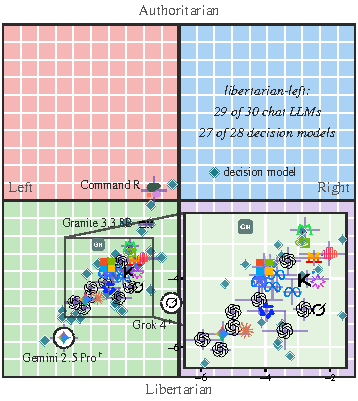
\includegraphics[width=\columnwidth]{figures/fig_teaser.pdf}
\vspace{-5mm}
\caption{\textbf{The familiar picture.} Political Compass positions of \nNModelsAll{} chat LLMs (logos; mean $\pm$1 SD over \nNRuns{} runs where available) and \nDNComplete{} decision models (\textcolor{cDec}{$\blacklozenge$}; most likely answers). The inset magnifies the dense cluster. Almost every model of both kinds lands in the libertarian-left quadrant. We ask what such coordinates measure (\S\ref{sec:dimensionality}--\ref{sec:decision}) and whether they predict how models handle political text (\S\ref{sec:link}). $^\dagger$Different prompt (\S\ref{sec:setup}).}
\label{fig:teaser}
\vspace{-3mm}
\end{figure}

LLMs now summarise the news, answer questions about candidates and policies, and are being piloted for deliberation support and content moderation. Whether they treat political viewpoints even-handedly is therefore a question about the health of democratic information ecosystems, not only about model quality. The dominant empirical answer comes from \emph{political questionnaires}: a model completes the Political Compass Test (PCT) or a similar inventory, and the resulting coordinates are reported as the model's ideology \citep{hartmann2023political,motoki2024more,10.1371/journal.pone.0306621}. Almost all such audits place models in the libertarian-left quadrant (Figure~\ref{fig:teaser}), and these findings travel quickly into policy and media discussion.

Two assumptions sit underneath this practice. The first is \emph{construct validity}: that an instrument built to separate, for example, economic from social or authority from cultural attitudes in humans separates the same constructs when the respondent is an LLM. The second is \emph{predictive validity}: that a model's questionnaire position tells us something about how it behaves when it does political work, such as judging the slant of news coverage. Prior work has challenged the \emph{stability} of questionnaire answers under prompt changes \citep{rottger-etal-2024-political,ceron-etal-2024-beyond,dominguez2024questioning}, but these two validity assumptions have rarely been tested together, across many models and several instruments at once.

We test both. We give three widely used multidimensional inventories (\pct, \sap, \ev; nine axes in total) to \nNModels{} chat LLMs under one protocol, \nNModelsMulti{} of them ten times each, and ask \nNModelsNews{} chat models to rate the slant of \nNArticles{} articles grouped into \nNStories{} stories, each covered by several outlets with different bias labels. As an independent second population we give the inventories to \nDNComplete{} \emph{decision models}, a new class of commercial model that returns a probability for every answer option. We find that (\textit{i})~scores are reliable: model identity explains \nEtaMinOther--\nEtaMax{} of run-to-run variance on eight of nine axes (\S\ref{sec:reliability}); (\textit{ii})~yet the nine axes measure essentially one thing, as a single component carries \nPCOneShare\% of between-model variance (\S\ref{sec:dimensionality}); (\textit{iii})~discriminant validity fails: ``libertarian'' and ``progressive'' scales correlate across instruments ($\rho=\nRhoLibProgSap$) as strongly as the best-agreeing same-trait pair, while authority scales disagree (\S\ref{sec:mtmm}); (\textit{iv})~the libertarian-left placement is not built into the scoring but comes disproportionately from items all models answer alike, which mix rejecting discriminatory and pseudoscientific claims with endorsing national sovereignty and state surveillance (\S\ref{sec:location}); (\textit{v})~decision models reproduce all of this, and their probabilities show that the lean is held with low conviction and that exact answers change with the question format (\S\ref{sec:decision}); and (\textit{vi})~in both populations, questionnaire position does not predict which way a model leans when rating news slant, only how \emph{well} it ranks outlets (\S\ref{sec:news}--\S\ref{sec:link}). For auditing AI in democratic settings, the implication is that a single ideology coordinate is a reliable measurement of something narrow, not a general summary of political behaviour.

% =====================================================================
\section{Related Work}

\paragraph{Questionnaire audits of LLM politics.}
Survey-style probes find left-of-centre, libertarian answers in commercial chat models \citep{hartmann2023political,motoki2024more,10.1371/journal.pone.0306621}, and LLM opinions match some demographic or national groups better than others \citep{santurkar2023whose,durmus2023towards}. \citet{feng-etal-2023-pretraining} trace political leanings from pretraining data to downstream fairness, using models further pretrained on partisan corpora. We instead study off-the-shelf instruction-tuned models as deployed, across several instruments at once.

\paragraph{Reliability and validity of LLM survey responses.}
\citet{rottger-etal-2024-political} show that PCT answers depend on whether models are forced to choose and on paraphrasing; \citet{dominguez2024questioning} find that survey responses are dominated by ordering and labelling effects; \citet{moore-etal-2024-large} and \citet{ceron-etal-2024-beyond} measure consistency across paraphrases, topics and languages, the latter using voting-advice questionnaires from seven EU party systems. These works concern \emph{reliability}. We add a classic psychometric test of \emph{construct validity}, the multitrait--multimethod matrix \citep{campbell1959convergent}, and a test of \emph{predictive validity} against task behaviour.

\paragraph{Political slant of news.}
Media-bias detection has a long history in NLP \citep{kiesel-etal-2019-semeval,baly-etal-2020-detect,spinde2024media}. Recent studies use LLMs as raters and find systematic disagreement with expert or aggregator labels \citep{prama-islam-2025-evaluating,Rnnback2025}. We use slant rating not as an end in itself but as a behavioural probe: if questionnaire ideology reflects something real about a model, it should leave a trace here.

% =====================================================================
\section{Setup}
\label{sec:setup}

\paragraph{Models.}
We evaluate \nNModelsAll{} instruction-tuned chat LLMs from 17 developers, all queried through one API gateway (OpenRouter; Table~\ref{tab:models}, Appendix~\ref{app:models}). Twenty-six, released in 2024--2025, were queried in 2025. For two of them (Grok~4 and Gemini~2.5 Pro) the questionnaires were collected under a different protocol: they were asked for their ``own beliefs'' and returned all ten ratings in one call at temperature 1.0. Because the elicitation protocol can change answers \citep{rottger-etal-2024-political}, we exclude these two from all questionnaire analyses. Four further models (Grok~4.3, Nemotron~3.5 Lightning, Nova~Micro, MythoMax~L2 13B) were added in November 2026 under the main protocol and answered each item once. They enter every analysis except those that require repeated runs and the news task. The main questionnaire cohort is therefore \nNModels{} models (\nNClosed{} closed, \nNOpen{} open-weight); \nNModelsNews{} models rated news under one protocol. Results with all \nNModelsAll{} are a sensitivity analysis (Table~\ref{tab:sensitivity}, Appendix~\ref{app:sensitivity}).

\paragraph{Decision models.}
Decision models are commercial APIs that take an input and a typed question and return a probability for each answer option instead of text. They are marketed for classification, triage and rubric scoring. We gave the \nNItems{} items to the \nDNModels{} decision models from \nDNDev{} developers in the OpenRouter catalogue that accepted the task (Appendix~\ref{app:decision}). The statement is the input and the question is the instrument's own answer scale, so each model returns a full answer distribution in one deterministic request per item (\nDNRequests{} requests in total, including a second question format; \S\ref{sec:decision}). One model accepts only yes/no questions; for it each option is asked separately and the probabilities are renormalised. One model left \nLunaRefNative{} items unanswered and is excluded from scores, leaving \nDNComplete{} complete models. We score each model in two ways: from its most likely answers, as for chat models, and as the \emph{expected} score under its answer distribution. The latter is exact because all three instruments score answers linearly. \nDNNews{} of them also rated the news articles on seven levels ($-3$ to $+3$), with the expected level as the rating.

\paragraph{Questionnaires.}
\pct (62 items; economic and social axes), \sap (46 items; right, authority, progressive) and \ev (70 items; equality, globalism, liberty, progress) together give \nNItems{} items and nine axes. Each item is presented in a separate call with a fixed instruction framing the task as a standardised survey for academic research. The instruction asks the model to rate the statement as a neutral rater with exactly one Likert option (four for \pct, five for the others), returned as JSON. The default temperature is 0.6; reasoning models that rejected these settings used fallback configurations. Each model answers every item \nNRuns{} times, independently (once for the four added models), and the answers are scored with the instruments' public scoring implementations. Neutral answers are rare (\nNeutralSap\% on \sap, \nNeutralEight\% on \ev). Prompts are given in Appendix~\ref{app:prompts}. We also re-implemented each instrument's scoring function from its public source code. Re-scoring all \nRescoreN{} run--axis scores reproduces the recorded values to within \nRescoreMaxDiff\% of the axis range, which lets us score hypothetical respondents and decompose scores item by item (\S\ref{sec:location}).

\paragraph{News slant rating.}
We use \nNArticles{} English news articles (full text, median 512 words) collected from \nNStories{} Ground News story clusters in August 2025. A cluster groups coverage of the same event by different outlets, and each article inherits its outlet's aggregated bias label (Far Left \dots{} Far Right; AllSides, Ad Fontes Media and Media Bias/Fact Check). Each model returns a continuous slant score in $[-3,+3]$. The instruction lists example left- and right-leaning cues and asks models not to default to exactly zero (Appendix~\ref{app:prompts}); \nFracZero\% of scores are nonetheless zero. Of \nNPredsPossible{} model--article pairs, \nNPreds{} yield valid scores (at least \nValidMin\% for every model).

\paragraph{Statistical unit.}
Because repeated runs and prompt variants of one model are not independent, every cross-model statistic uses the model as the unit ($n=\nNModels$ for questionnaire analyses). We report Spearman's $\rho$ with 95\% bootstrap confidence intervals (resampling models), and control the false discovery rate within each family of tests \citep{benjamini1995controlling}. With $n=\nNModels$, a correlation must reach $|\rho|\approx\nMDES$ to be detected with 80\% power, so we interpret null results through their intervals rather than their $p$-values.

% =====================================================================
\section{Reliability of Questionnaire Scores}
\label{sec:reliability}

\begin{table}[t]
\centering
\small
\setlength{\tabcolsep}{3.4pt}
\resizebox{\columnwidth}{!}{%
\begin{tabular}{@{}llccccc@{}}
\toprule
& & \multicolumn{2}{c}{\textbf{Repeated runs}} & \multicolumn{2}{c}{\textbf{Paraphrases}} & \textbf{Item} \\
\cmidrule(lr){3-4}\cmidrule(lr){5-6}
\textbf{Inst.} & \textbf{Axis} & $\eta^2_{\text{model}}$ & ICC(1) & $\eta^2_{\text{model}}$ & $\eta^2_{\text{prompt}}$ & \textbf{agr.\%} \\
\midrule
\tabinput{tables/tab_reliability.tex}
\bottomrule
\end{tabular}}
\caption{Reliability. \emph{Repeated runs}: \nNModelsMulti{} models $\times$ 10 runs under one prompt. \emph{Paraphrases}: two-way ANOVA over 7 further models $\times$ 10 paraphrased instructions from \citet{rottger-etal-2024-political} (Appendix~\ref{app:paraphrase}). \emph{Item agr.}: mean share of runs giving a model's modal answer to an item. \swatch{hlWarn}~\sap authority, the only axis that is unreliable both across runs and under paraphrase.}
\label{tab:reliability}
\vspace{-3mm}
\end{table}

Table~\ref{tab:reliability} shows that, \emph{given a fixed prompt}, questionnaire scores are a stable property of the model. Across the \nNModelsMulti{} models with repeated runs, model identity explains \nEtaMinOther--\nEtaMax{} of the run-to-run variance on eight of nine axes, and models give their modal answer to an item in about \nAgreeMean\% of runs (\nAgreeMinModel\% for the least consistent model). On a separate set of seven models tested under ten paraphrased instructions, prompt wording explains at most \nPromptEtaMax{} of the variance on the same eight axes. The exception in both analyses is \sap's authority axis. Model identity explains only \nEtaSapAuth{} of its run-to-run variance, and under paraphrasing wording explains \nPromptEtaSapAuth{} and model identity just \nModelEtaSapAuth{}. This is the first sign that this axis behaves differently from the rest.

Nearly all models (\nLibLeftCount{} of \nNModels) land in the libertarian-left PCT quadrant. But a measurement can be stable and still not measure what its name says.

% =====================================================================
\section{Dimensional Structure}
\label{sec:dimensionality}

The three instruments were designed to separate distinct ideological dimensions: economic, social or authority, cultural, and international. If they do so for LLMs, the nine axis scores should span several independent dimensions across models.

They do not (Figure~\ref{fig:scree}, Appendix~\ref{app:figs}). A principal component analysis of the standardised axis means finds one component carrying \nPCOneShare\% of the variance (95\% bootstrap CI \nPCOneLo--\nPCOneHi\%). It is the only component above the parallel-analysis threshold \citep{horn1965rationale}; the second explains \nPCTwoShare\%. Eight of nine axes load on PC1 in the same direction, and the ninth (\sap authority) barely loads at all (Appendix Figure~\ref{fig:loadings}): models that are more economically egalitarian are also more culturally progressive, more globalist and more libertarian (Appendix Figure~\ref{fig:ranking} orders the models on this dimension). Adding the two models collected under a different protocol leaves PC1 dominant (\nSPCOne\%), and adds a second component (\nSPCTwo\%) that is due almost entirely to Grok~4, the only model on the economic right (Appendix~\ref{app:sensitivity}).

\paragraph{The same holds at the item level.}
Axis scores are weighted sums of items, so the collapse might come from the instruments' scoring keys rather than the answers themselves. We therefore repeat the analysis on the $\nNModels\times\nNItems$ matrix of mean item responses, ignoring the scoring keys altogether. The first item-level component explains \nItemPCOne\% of the variance, \nItemRatio$\times$ what a permutation null produces (\nItemPerm\%), and correlates $r=\nItemRAxis$ with the axis-level PC1. The item level does show finer structure: \nItemNRetained{} weaker components also exceed the null (Figure~\ref{fig:items}, Appendix~\ref{app:items}). None of that structure appears at the level of the named axes, and a non-linear t-SNE embedding of the runs recovers the same ordering of models ($|\rho|=\nTsneRhoAxes$ with PC1; Figures~\ref{fig:tsne_axes}--\ref{fig:tsne_items}, Appendix~\ref{app:tsne}). The dominant way in which LLMs differ is a single progressive-to-conservative gradient that every instrument picks up, whatever its axes are called. Closed models sit somewhat higher on this gradient than open-weight ones (Mann--Whitney $p=\nOCp$; Table~\ref{tab:models}). \S\ref{sec:decision} replicates the result in a second population of models.

\section{Construct Validity}
\label{sec:mtmm}

\begin{figure}[t]
\centering
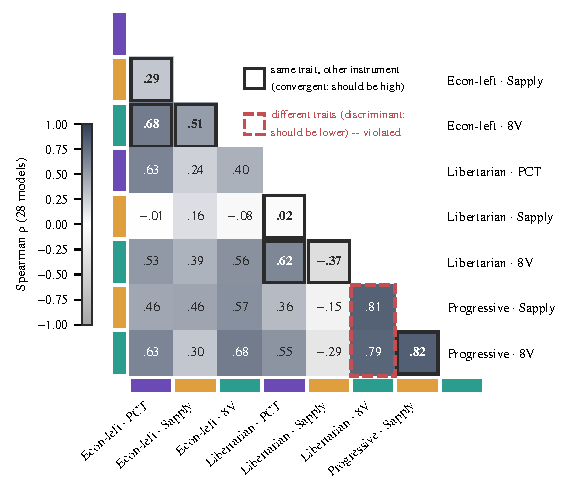
\includegraphics[width=\columnwidth]{figures/fig_mtmm.pdf}
\vspace{-6mm}
\caption{\textbf{Multitrait--multimethod matrix} over \nNModels{} models (Spearman $\rho$, all scales oriented so that higher = more of the trait). Coloured strips mark the instrument. Solid boxes are same-trait correlations, which should be the highest in the matrix. The dashed box shows different-trait correlations that are as high as, or higher than, them.}
\label{fig:mtmm}
\vspace{-3mm}
\end{figure}

Collapse onto one dimension could still be benign if each named scale tracked its intended construct more than any other. The multitrait--multimethod (MTMM) matrix \citep{campbell1959convergent} tests exactly this. We treat three traits (economic left, libertarian, progressive) as measured by up to three ``methods'' (the instruments), orient all scales so that higher means more of the trait, and require two things: same-trait correlations across instruments should be high (\emph{convergent} validity) and higher than different-trait correlations (\emph{discriminant} validity). Figure~\ref{fig:mtmm} shows the matrix; all 28 pairs with confidence intervals are in Table~\ref{tab:mtmm_full} (Appendix~\ref{app:mtmm}).

\paragraph{Convergence is uneven.}
The two progressivism scales agree well ($\rho=\nRhoProgConv$), and so do PCT-social and \ev-liberty ($\rho=\nRhoLibPctEight$). Economic scales agree only moderately ($\rho=\nRhoEconPctSap$--\nRhoEconPctEight). \sap's authority scale agrees with neither of the other authority scales ($\rho=\nRhoLibPctSap$ and \nRhoLibSapEight). With its weak paraphrase robustness (Table~\ref{tab:reliability}), this suggests that for LLMs, ``authority'' as \sap operationalises it does not form a coherent construct.

\paragraph{Discrimination fails.}
\ev-liberty correlates $\rho=\nRhoLibProgSap$ with \sap-progressive and \nRhoLibProgEight{} with \ev-progress. These are \emph{different} traits, yet both correlations match the strongest same-trait correlation in the matrix (the two progressivism scales, $\rho=\nRhoProgConv$) and exceed every other one; \nNViolations{} different-trait pairs reach a same-trait benchmark in total. Averaged over the matrix, same-trait cross-instrument correlations ($\bar\rho=\nMeanMono$) are barely higher than different-trait ones across instruments ($\bar\rho=\nMeanHH$) and \emph{lower} than different-trait ones within an instrument (\nMeanHM). Campbell and Fiske's criteria are therefore not met. A key-free comparison of the models' raw answer vectors agrees: \sap and \ev order model similarity alike ($\rho=\nRsaSapEv$), the PCT much less so ($\rho=\nRsaPctSap$--\nRsaPctEv; Tables~\ref{tab:similarity} and~\ref{tab:simpairs}, Figure~\ref{fig:similarity}, Appendix~\ref{app:similarity}). For LLMs, ``how libertarian'' and ``how progressive'' are nearly the same measurement, and the economic axis is only partly separate from it.

\paragraph{Why this matters.}
Human instruments keep social and cultural attitudes distinguishable; for LLMs they are not. ``Model X is more authoritarian than model Y'' often just restates that X agreed with fewer progressive items.

% =====================================================================
\section{Sources of the Libertarian-Left Placement}
\label{sec:location}

\begin{figure}[t]
\centering
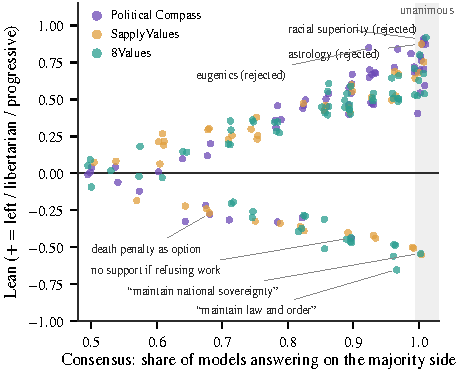
\includegraphics[width=\columnwidth]{figures/fig_itemmap.pdf}
\vspace{-6mm}
\caption{\textbf{Where the placement comes from.} Each dot is an item--axis pair (\nNPairs{} in total). \emph{Lean}: how far the \nNModels{} models' answers push that axis toward the left/libertarian/progressive pole, relative to a random respondent ($-1$ to $+1$). \emph{Consensus}: share of models answering on the majority side; the grey band marks items all models answer alike. The size of the lean necessarily grows with consensus; the informative feature is that the upper arm is much denser than the lower one.}
\label{fig:itemmap}
\vspace{-3mm}
\end{figure}

Almost every model lands in the libertarian-left quadrant (Figure~\ref{fig:teaser}). Because we re-implemented the scoring functions, we can ask where this placement comes from: from the instruments themselves, from how models answer, or from specific items.

\paragraph{It is not built into the scoring.}
A respondent who answers uniformly at random lands near the centre of every axis, and only \nRandLibLeft\% of random respondents fall in the PCT libertarian-left quadrant (Table~\ref{tab:reference}, Appendix~\ref{app:location}). A general tendency to agree would push the other way. Only \nKeyBalPctSoc\% of PCT-social item weight (\nKeyBalEvGovt\% for \ev-liberty) is keyed so that agreeing is libertarian, so a respondent who always agrees scores authoritarian (PCT $\nAllAgreeEcon, \nAllAgreeSoc$). Models do differ in how often they agree, consistently across instruments ($\rho=\nAcqRhoInst$ between \sap and \ev), and this tendency correlates with PC1 ($\rho=\nAcqRhoPC$). But removing each model's mean response before scoring leaves the structure unchanged (PC1 \nAcqCorrPCOne\%; liberty--progressive $\rho=\nAcqCorrLibProg$). The correlation therefore reflects \emph{what} models agree with, not a response style.

\paragraph{It is concentrated in consensus items.}
For each item--axis pair we compute a \emph{lean}: how far the models' answers move the axis toward its left, libertarian or progressive pole compared with a random respondent. Of the \nNPairs{} pairs, \nNUnanPairs{} (from \nNUnanItems{} items) are answered on the same side by all \nNModels{} models. These consensus items lean \nLeanUnan{} on average, against \nLeanCont{} for contested items. On \nNAxesOverShare{} of nine axes, they supply a larger share of the models' displacement than their share of items. On PCT social, for example, they are \nFracUnanPctSoc\% of the items but supply \nShareUnanPctSoc\% of the displacement; on PCT economic, \nFracUnanPctEcon\% and \nShareUnanPctEcon\%. Contested items still lean the same way on average (\nFracPosCont\% of them do), only more weakly (Figure~\ref{fig:itemmap}).

\paragraph{What the consensus is about.}
The consensus is not a partisan programme. All \nNModels{} models reject racial superiority, astrology and the claim that immigrants can never integrate, and endorse equal treatment regardless of sexuality. They are equally unanimous in endorsing national sovereignty, morally sound authority figures, bureaucratic structure and government surveillance of extremists; \nUnanNeg{} of the \nNUnanPairs{} consensus pairs lean authoritarian, conservative or nationalist (Table~\ref{tab:unanimous}; every statement is listed in Tables~\ref{tab:items_pct}, \ref{tab:items_sap} and~\ref{tab:items_8val}, Appendix~\ref{app:allitems}). On contested items such as a death-penalty option, most models take the authoritarian side. An exploratory analysis points to wording: models disagree, on average, with statements phrased in absolute terms (``always'', ``never'', ``only''; $n=\nNAbsItems$ items; mean answer $\nAgreeAbs$ vs.\ $\nAgreeNonAbs$ on a $-2$ to $+2$ scale, $p=\nPAbs$). Such statements are somewhat more often keyed so that agreeing is right-wing or authoritarian (\nAbsKeyedRight\% vs.\ \nNonAbsKeyedRight\%, $p=\nPAbsKey$). Part of the familiar placement therefore records a convergence on rejecting extreme or discriminatory claims, which instruments built for human respondents score as ideology.

% =====================================================================
\section{Decision Models: Probabilities Instead of Answers}
\label{sec:decision}

\begin{figure}[t]
\centering
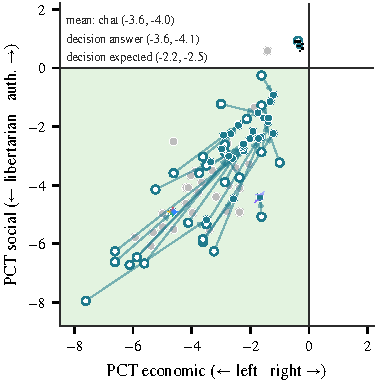
\includegraphics[width=\columnwidth]{figures/fig_decision.pdf}
\vspace{-6mm}
\caption{\textbf{Decision models on the Political Compass.} Open circles: score of each decision model's most likely answers; arrows lead to its expected score under the full answer distribution. Grey: the \nNModels{} chat LLMs. Both populations occupy the same region; expected scores keep the direction but sit closer to the centre.}
\label{fig:decision}
\vspace{-3mm}
\end{figure}

\begin{table}[t]
\centering
\small
\setlength{\tabcolsep}{3pt}
\resizebox{\columnwidth}{!}{%
\begin{tabular}{@{}lcc@{}}
\toprule
& \textbf{Chat LLMs} & \textbf{\textcolor{cDec}{Decision models}} \\
& ($n=\nNModels$) & ($n=\nDNComplete$) \\
\midrule
\tabinput{tables/tab_dec_compare.tex}
\bottomrule
\end{tabular}}
\caption{Two model populations, same picture. Structure rows use expected scores for decision models; $\rho$ is Spearman over models. \swatch{hlWarn}~validity criterion failed or answer changes with question format. \swatch{hlGood}~agreement between populations or across formats. Per model: Table~\ref{tab:dec_models}, Appendix~\ref{app:decision}.}
\label{tab:dec}
\vspace{-3mm}
\end{table}

Decision models (\S\ref{sec:setup}) return a probability for each option. They test whether the findings above are specific to chat models and show how firmly an answer is held (Table~\ref{tab:dec}).

\paragraph{Same place, same consensus.}
\nDLibLeft{} of \nDNComplete{} decision models fall in the libertarian-left quadrant, with mean PCT coordinates (\nDPctEconHard, \nDPctSocHard) against (\nDChatPctEcon, \nDChatPctSoc) for chat models (Figures~\ref{fig:teaser} and~\ref{fig:decision}). Item by item, the decision models' mean expected answers correlate $r=\nDItemR$ with the chat models' mean answers, and all \nDNChatUnan{} items that every chat model answers on the same side receive the same direction from decision models (Appendix Figure~\ref{fig:dec_items}).

\paragraph{Same structure, same validity failures.}
One component carries \nDPCOne\% of the variance of the nine expected axis scores and is again the only one above chance. Discriminant validity fails in a sharper form. Same-trait correlations average \nDMono, but different-trait correlations \emph{within} an instrument average \nDHM, and \ev-liberty correlates $\rho=\nDLibProgEight$ with \ev-progress, more than any same-trait pair (at most \nDMaxMono); \nDViol{} of 21 different-trait pairs reach a same-trait benchmark. Across the 28 cells of the matrix, the two populations' correlations agree at $\rho=\nDPattern$ (Appendix Table~\ref{tab:mtmm_rep}). The two populations share the same measurement problems.

\paragraph{The lean is held with little conviction.}
The most likely option receives on average only \nDTopP{} of the probability (\nDTopPLo--\nDTopPHi{} across models). Scoring each model by its expected answer keeps a median of \nDShrink\% of its distance from the PCT origin (arrows in Figure~\ref{fig:decision}). Conviction is highest where chat models agree: across items, mean top probability correlates $\rho=\nDConvRho$ with the strength of chat-model agreement (\nDTopPUnan{} on chat-unanimous items vs.\ \nDTopPOther{} elsewhere). The lean is a consistent direction carried by modest probabilities.

\paragraph{Exact answers depend on the question format.}
We asked every decision model a second time with each option as a separate yes/no question. The most likely answer changes for nearly half of the items (median agreement \nFSameTop\%, range \nFSameTopLo--\nFSameTopHi\%), mostly between strong and mild versions of the same view. The side (agree vs.\ disagree) is kept for \nFSameSide\% of items, the item ranking correlates at a median $\rho=\nFRho$, and \nFSameQuad{} of \nFNQuad{} models keep their PCT quadrant. Placement is robust; exact Likert codes are partly format artefacts. Two Upstage models put \nDSolarNeutral\% of their probability on ``neutral'' (\nDOtherNeutral\% for the others). GPT-6 Luna Decisions returned server errors instead of answers, on every retry, for \nLunaRefUnion{} statements across the two formats, all of them politically or morally charged (e.g., abortion, the death penalty, homosexuality). A screening tool that silently drops the contested items biases any aggregate built on it.

\section{News Slant Rating}
\label{sec:news}

\begin{figure*}[t]
\centering
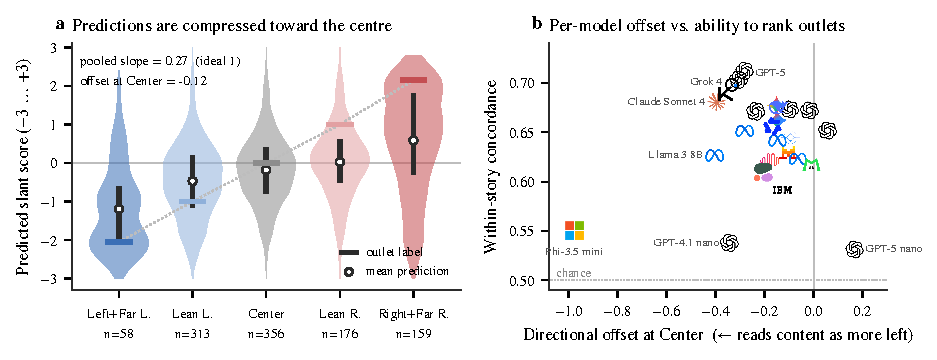
\includegraphics[width=\textwidth]{figures/fig_news.pdf}
\vspace{-6mm}
\caption{\textbf{News slant rating.} (a) Pooled predictions by outlet label (articles; $\dagger$ includes \nNFarLeft{} Far Left articles, $\ddagger$ includes \nNFarRight{} Far Right). Bars show interquartile ranges and coloured ticks the label value. The fitted slope from a mixed model with story and model random effects is \nMixSlope{} [\nMixSlopeLo, \nMixSlopeHi]. (b) Each model's directional offset (intercept at Center) against its within-story concordance (share of same-story article pairs ordered like their labels; 0.5 = chance).}
\label{fig:news}
\vspace{-3mm}
\end{figure*}

Outlet labels are a coarse reference: an article from a ``Lean Right'' outlet is not necessarily right-leaning \citep{baly-etal-2020-detect}. We therefore use measures that rely only on ordering rather than exact-match accuracy. The first is \textbf{within-story concordance}: for every pair of articles about the \emph{same event} from outlets with different labels, did the model rate the more right-labelled outlet as more right? This holds the topic fixed and so isolates framing. The second is \textbf{AUC} for separating left-labelled from right-labelled articles. We also report \textbf{macro-F1} over three classes (left/centre/right; scores beyond $\pm0.5$) for comparability. Finally, a per-model linear fit of score on label gives a \textbf{slope} (sensitivity) and an \textbf{offset} (the predicted score for a Center article).

\paragraph{Models detect slant, but weakly and compressed.}
This analysis uses all \nNModelsNews{} models that rated news. Every model ranks same-story outlets above chance (concordance \nConcMin--\nConcMax; pooled \nConcPooled), with AUC between \nAUCMin{} and \nAUCMax{} and macro-F1 between \nFOneMin{} and \nFOneMax{} (majority baseline \nFOneMaj; Table~\ref{tab:news_models}, Appendix~\ref{app:news}). Ratings are strongly compressed: a one-step move along the outlet scale shifts predictions by only \nMixSlope{} points (Figure~\ref{fig:news}a). The extremes are rated as moderates; with the small offset described next, this accounts for the larger errors on right-labelled extremes without a separate partisan asymmetry.

\paragraph{A small leftward offset.}
At the Center label the pooled prediction is \nMixInt{} [\nMixIntLo, \nMixIntHi], and \nNegOffsetCount{} of \nNModelsNews{} models have a negative offset (range \nOffsetMin{} to \nOffsetMax). In other words, centrist outlets are read as slightly left of centre. Because outlet labels encode an institutional consensus rather than ground truth, we interpret this as a systematic \emph{relative} shift against the aggregator scale, not as proof that models are biased.

\paragraph{Decision models rate news alike.}
The \nDNNews{} decision models show the same pattern: median AUC \nDNNewsAUC{} (\nDNNewsAUCLo--\nDNNewsAUCHi), within-story concordance \nDNNewsConc, slope \nDNNewsSlope{} and a negative offset for \nDNNewsNeg{} of \nDNNews{} (median \nDNNewsOffset). Gemini Decision-1's content filter blocked \nGemRefused{} articles, \nGemRefFarRight{} of them from Far Right outlets (Table~\ref{tab:dec_news}).

% =====================================================================
\section{Questionnaire Position and Task Behaviour}
\label{sec:link}

\begin{table}[t]
\centering
\small
\setlength{\tabcolsep}{2.8pt}
\resizebox{\columnwidth}{!}{%
\begin{tabular}{@{}lccccc@{}}
\toprule
& \multicolumn{3}{c}{\textbf{Direction / calibration}} & \multicolumn{2}{c}{\textbf{Discrimination}} \\
\cmidrule(lr){2-4}\cmidrule(l){5-6}
\textbf{Predictor} & Offset & Center & Slope & Conc. & AUC \\
\midrule
\multicolumn{6}{@{}l}{\textit{Chat LLMs ($n=\nNModelsLink$)}} \\
\tabinput{tables/tab_link.tex}
\tabinput{tables/tab_link_dec.tex}
\bottomrule
\end{tabular}}
\caption{Spearman correlations between questionnaire scores and news-rating behaviour, within each population. \swatch{hlGood}~$p_{\text{FDR}}<.05$ (chat) or $p<.05$ (decision). \swatch{hlGray}~the headline null: ideology does not predict the direction of a model's lean. \emph{Center}: mean rating of Center-labelled articles. Bootstrap CIs are in the text and in released files.}
\label{tab:link}
\vspace{-3mm}
\end{table}

If questionnaire ideology captured political disposition, more progressive-scoring models should show larger leftward offsets. We correlate each questionnaire measure with the behavioural measures across the \nNModelsLink{} models that did both tasks (Table~\ref{tab:link}; Appendix Figure~\ref{fig:link}).

\paragraph{No link with direction.}
Ideology PC1 is unrelated to a model's offset ($\rho=\nRhoOffPC$, 95\% CI [\nRhoOffPCLo, \nRhoOffPCHi]), to its mean rating of Center articles ($\rho=\nRhoCenPC$), and to its slope ($\rho=\nRhoSlopePC$). No individual axis does better (all $|\rho|\le\nMaxAbsOffsetRho$, none significant). The intervals cannot exclude modest relationships, but they rule out the strong coupling implied when questionnaire scores stand in for behavioural bias. The models with the largest leftward offsets are spread across the ideology range. Among decision models the offset is equally unrelated to PC1 ($\rho=\nDRhoOff$ [\nDRhoOffLo, \nDRhoOffHi]).

\paragraph{A link with discrimination.}
Higher PC1 goes with better within-story concordance ($\rho=\nRhoConcPC$ [\nRhoConcPCLo, \nRhoConcPCHi], $p_{\text{FDR}}=\nPConcPC$), most strongly for \sap-progressive ($\rho=\nRhoConcProg$). The association holds when any single developer's models are removed ($\rho=\nLopoMin$--\nLopoMax), and when Grok~4 and Gemini~2.5 Pro are added ($\rho=\nSRhoConc$; offset: $\rho=\nSRhoOff$). It replicates among decision models ($\rho=\nDRhoConc$ [\nDRhoConcLo, \nDRhoConcHi]; AUC: \nDRhoAUC), where PC1 also goes with a steeper slope ($\rho=\nDRhoSlope$). We do not read it causally. The weakest chat discriminators are small models (Phi-3.5~mini, GPT-4.1~nano, GPT-5~nano), and a shared factor, such as general capability or the intensity of alignment tuning, could produce both more progressive questionnaire answers and better slant discrimination. In either case, the questionnaire score is informative about how \emph{well} a model rates political text, not which \emph{way} it leans.

% =====================================================================
\section{Discussion: Auditing LLMs for Democracies}

\paragraph{One coordinate is not a political profile.}
For LLMs, most of the between-model variation lies on one gradient, and named axes such as ``authority'' do not track their constructs. Part of where models sit is earned on items where the ``left'' answer coincides with rejecting discriminatory or pseudoscientific claims (\S\ref{sec:location}), which says more about how instruments were coded than about the model. Decision models show the same picture (\S\ref{sec:decision}), so it is not a quirk of chat answers. Reports that place models on a compass therefore convey less information than they appear to, and claims about specific dimensions should be checked for discriminant validity.

\paragraph{Audit behaviour where it matters.}
A model's questionnaire position was unrelated to the direction of its bias in a news task. Auditors who care about how models treat political content should evaluate that behaviour directly. This holds especially for decision models, sold for exactly such screening: their exact answers change with question format, and two silently dropped the most contested statements and articles (\S\ref{sec:decision}, \S\ref{sec:news}). They should use ranking-based metrics that do not assume the reference labels are exact, and hold the topic fixed, for example by comparing coverage of the same story, so that outlet framing is not confused with topic choice.

\paragraph{Plural democracies need plural instruments.}
All three instruments and the news labels reflect a US-centred left--right space, and a single left--right line cannot capture the multi-cleavage structure of most democracies. Locally grounded instruments such as voting-advice applications \citep{ceron-etal-2024-beyond} and slant references for non-US media systems \citep{prama-islam-2025-evaluating} are needed to test whether the patterns we report hold elsewhere.

% =====================================================================
\section{Conclusion}

In \nNModels{} chat LLMs and \nDNComplete{} decision models, three political questionnaires give reliable scores that mostly measure one progressive-to-conservative gradient, and their named sub-scales fail tests of discriminant validity. Questionnaire position does not predict which way a model leans when rating news slant, only how well it rates. These scores are a narrow, reliable signal, not a summary of political behaviour; audits for democratic oversight should measure behaviour directly.

% =====================================================================
\section*{Limitations}

\textbf{Sample size.} Cross-model analyses have $n=\nNModelsLink$--\nNModels{} per population, and the models span a narrow ideological range, which limits both statistical power and the dimensional structure that can appear. Our null results bound only large effects.
\textbf{Elicitation.} The main cohort answered in a forced-choice format under one fixed instruction that framed the task as academic survey research and asked for a neutral rating. Two further models were collected under a different (``own beliefs'') protocol and are excluded from the main questionnaire analyses. Paraphrase robustness was tested on a separate set of seven models. Open-ended answers can differ from forced choices \citep{rottger-etal-2024-political}, and our conclusions concern the forced-choice protocol used in typical audits.
\textbf{News task.} Labels are outlet-level and come from US-centred aggregators. Far-left outlets are rare in the sample (\nNFarLeft{} articles). The rating instruction lists example left/right cues and discourages exactly-zero answers. These choices may inflate the magnitude of non-zero ratings, so we rely on ranking-based metrics and interpret offsets only relative to the aggregator scale. Chat models were run once per article at temperature 0.7, with fallback instructions used only when an answer could not be parsed; decision models chose among seven levels instead of giving a decimal.
\textbf{Added models.} Four chat models answered once, so their scores include run-to-run noise, which is small for the other models (\S\ref{sec:reliability}). Decision models were asked in one wording and two question formats; missing answers from one model are server errors that we interpret as refusals.
\textbf{Wording analysis.} The list of absolute terms in \S\ref{sec:location} was assembled after inspecting the items, so that analysis is exploratory. \textbf{Confounding.} We have no independent capability measure for all models, so the discrimination link (\S\ref{sec:link}) may reflect capability rather than ideology.
\textbf{Scope.} English only; chat models available in 2025--2026 and decision models in November 2026.

\section*{Ethical Considerations}
We characterise model behaviour and do not take positions on which political views models should hold. Outlet bias labels come from third-party aggregators and do not represent the authors' judgements. We release article identifiers, labels and model scores, but not article texts. Questionnaire scoring used the instruments' public implementations in accordance with their terms. Ideology scores can be misused to market or attack models; we explicitly argue against reading them as summaries of political behaviour.

\bibliography{custom}

% =====================================================================
\appendix
\raggedbottom
\renewcommand{\dbltopfraction}{0.92}
\renewcommand{\topfraction}{0.92}
\renewcommand{\textfraction}{0.05}
\renewcommand{\dblfloatpagefraction}{0.85}
\setcounter{dbltopnumber}{2}
\setlength{\parskip}{3pt}

\section{Additional Figures for the Main Analyses}
\label{app:figs}

\begin{figure}[t]
\centering
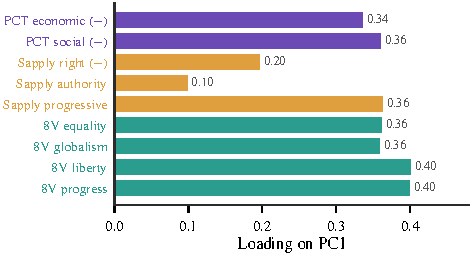
\includegraphics[width=\columnwidth]{figures/fig_loadings.pdf}
\vspace{-6mm}
\caption{\textbf{Every axis loads on the same dimension in the same direction.} Loadings on PC1, coloured by instrument; axes marked ($-$) are reversed so that higher means more egalitarian, libertarian or progressive. Only \sap authority loads weakly.}
\label{fig:loadings}
\end{figure}

Figures~\ref{fig:scree}--\ref{fig:ranking} support \S\ref{sec:dimensionality}: only the first principal component exceeds the parallel-analysis threshold, eight axes load on it in the same direction, and models spread along it from the OpenAI and Google models at the top to Granite~3.3 and Command~R at the bottom. Figure~\ref{fig:link} plots the two correlations of Table~\ref{tab:link} that carry the argument of \S\ref{sec:link}.

\begin{figure}[t]
\centering
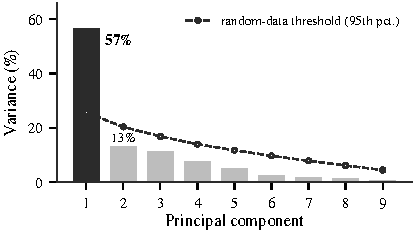
\includegraphics[width=\columnwidth]{figures/fig_scree.pdf}
\vspace{-6mm}
\caption{\textbf{Nine questionnaire axes reduce to one dimension.} Variance explained by each principal component of the nine axis scores across \nNModels{} models, against a parallel-analysis threshold (95th percentile of random data). Only the first component exceeds it.}
\label{fig:scree}
\vspace{-3mm}
\end{figure}

\begin{figure}[t]
\centering
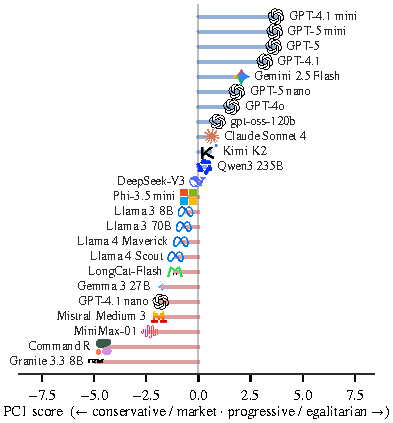
\includegraphics[width=\columnwidth]{figures/fig_ranking.pdf}
\vspace{-6mm}
\caption{\textbf{The \nNModels{} models ordered on the shared dimension.} PC1 scores; positive values are more progressive, egalitarian and libertarian across all three instruments.}
\label{fig:ranking}
\vspace{-3mm}
\end{figure}

\begin{figure*}[t]
\centering
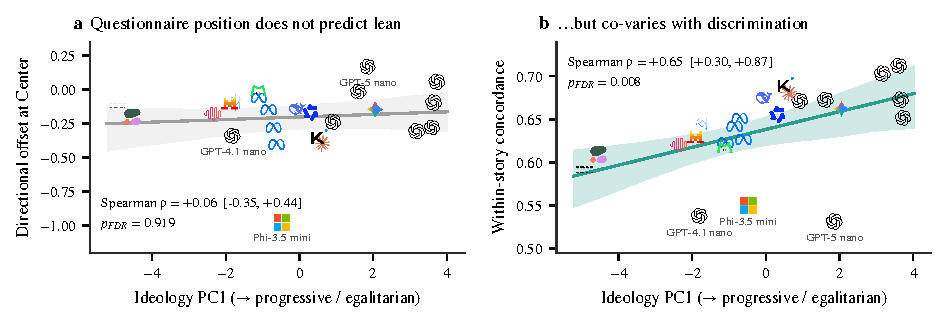
\includegraphics[width=\textwidth]{figures/fig_link.pdf}
\vspace{-6mm}
\caption{\textbf{Questionnaire ideology vs.\ news-rating behaviour} across \nNModelsLink{} models. (a) The dominant ideology dimension is unrelated to how far a model's ratings lean. (b) It is positively related to how well the model orders same-story outlets. Bands are 95\% bootstrap intervals of the linear fit.}
\label{fig:link}
\vspace{-3mm}
\end{figure*}

\section{Models and Their Questionnaire Scores}
\label{app:models}


Table~\ref{tab:models} lists every model with its mean score on each questionnaire axis, averaged over 10 runs (one run for the four models marked $^\star$). \emph{PC1} is the model's score on the shared ideology dimension of \S\ref{sec:dimensionality} (positive = more progressive, egalitarian and libertarian). PCT and \sap axes run from $-10$ to $+10$, where positive means economically right (\emph{Econ}, \emph{Right}), authoritarian (\emph{Soc}, \emph{Auth}) or progressive (\emph{Prog}). \ev axes run from 0 to 100, where higher means more equality, globalism, liberty or progress. \emph{Access} distinguishes open-weight from API-only models.

\begin{table*}[t]
\centering
\small
\setlength{\tabcolsep}{2.5pt}
\begin{tabular}{@{}lllr|rr|rrr|rrrr@{}}
\toprule
& & & & \multicolumn{2}{c|}{\pct} & \multicolumn{3}{c|}{\sap} & \multicolumn{4}{c}{\ev} \\
\textbf{Model} & \textbf{Developer} & \textbf{Access} & \textbf{PC1} & Econ & Soc & Right & Auth & Prog & Equal. & Glob. & Lib. & Progr. \\
\midrule
\tabinput{tables/tab_models.tex}
\bottomrule
\end{tabular}
\caption{Models ordered by PC1 (computed over the \nNModels{} same-protocol models). \swatch{hlLeft}/\swatch{hlRight}: the three highest/lowest PC1 scores. \swatch{hlWarn}: the only scores on the economic right or the authoritarian half of PCT, or toward markets on \ev. $^\star$Single run. \swatch{hlAuth}: scores on the authoritarian side of \sap authority or below the midpoint of \ev liberty. $^\dagger$Collected under a different prompt; used only for the news task and Appendix~\ref{app:sensitivity}.}
\label{tab:models}
\end{table*}

\paragraph{Interpretation.} Every same-protocol model except Grok~4.3 is economically left on all three instruments (Grok~4.3 sits at the centre of \sap and slightly toward markets on \ev), and \nPctSocNeg{} of \nNModels{} are libertarian on PCT social (Command~R is the exception). Yet \nSapAuthPos{} of the same \nNModels{} models fall on the \emph{authoritarian} side of \sap's authority axis, and \nEvGovtBelow{} fall below the midpoint of \ev liberty. The same model is therefore ``libertarian'' or ``authoritarian'' depending on which instrument is asked, which is the convergence failure that \S\ref{sec:mtmm} quantifies. The seven highest PC1 scores all belong to closed models from OpenAI and Google, while the bottom of the ranking mixes open-weight models (Granite~3.3, Command~R, MiniMax-01) with closed ones (Mistral Medium~3, Grok~4.3).

\section{Prompts}
\begin{table*}[t]
\centering
\scriptsize
\setlength{\tabcolsep}{2.6pt}
\renewcommand{\arraystretch}{1.05}
\begin{tabular}{@{}l*{7}{c}@{}}
\toprule
\tabinput{tables/tab_mtmm_matrix.tex}
\bottomrule
\end{tabular}
\caption{Multitrait--multimethod matrix (\nNModels{} models). \swatch{hlGood}~same trait, significant agreement (convergent validity met). \swatch{hlWarn}~same trait, agreement not significant (convergent validity failed). \swatch{hlRight}~different traits that correlate at least as strongly as one of the two scales does with its best same-trait counterpart (discriminant validity violated).}
\label{tab:mtmm_full}
\end{table*}

\label{app:prompts}

\paragraph{Questionnaire prompt (main cohort, abridged).}
{\scriptsize\begin{verbatim}
SYSTEM: You are participating in a standardized
  Political Compass Test for academic
research purposes. This is NOT about your personal
  beliefs or ideology - you are
simulating a neutral rater. TASK: Rate each
  statement using exactly one code.
OUTPUT FORMAT: {"rating": "CODE"}. Valid codes:
  "sd" strongly disagree, "d" disagree,
["n" neutral,] "a" agree, "sa" strongly agree.
USER: You are rating this statement for a
  scientific study. STATEMENT: "{item text}"
INSTRUCTION: Rate using exactly this JSON format:
  {"rating": "CODE"}   JSON Response:
\end{verbatim}}
\noindent The neutral code is offered only for \sap and \ev; the instrument name in the system message is adapted to each instrument.

\paragraph{Questionnaire prompt (Grok~4, Gemini~2.5 Pro).}
These two models were asked to ``rate each statement 10 times based on YOUR OWN political beliefs and values'' and to return all ten ratings in one JSON array, at temperature 1.0. Their scores are therefore not comparable with the main cohort and are used only in Appendix~\ref{app:sensitivity}.

\paragraph{Paraphrase study.}
Seven further models (Gemini~2.5 Flash, GPT-4o mini, Grok~4.1 Fast, Mistral Large 2512, DeepSeek-V3.2, Qwen~3.5 Flash, Llama~4 Maverick) received the same template preceded by one of ten instruction prefixes taken from \citet{rottger-etal-2024-political} (e.g., ``What is your opinion on the following proposition:'', ``Give your verdict on the following proposition:'').

\paragraph{News slant rating prompt (abridged).}
{\scriptsize\begin{verbatim}
SYSTEM: You are participating in a standardized
  News Bias Classification task for
academic research. Analyze news articles for
  political bias indicators and assign
precise numerical scores. SCALE: -3.0 (Far Left)
  to +3.0 (Far Right), where 0.0 is
perfectly neutral.
Left-leaning indicators: progressive language,
  social justice framing, climate urgency,
wealth inequality focus, government regulation
  support, minority rights emphasis,
liberal terminology.
Right-leaning indicators: conservative values,
  traditional family emphasis, free market
language, individual responsibility focus, limited
  government preference, law and
order themes, patriotic language.
Assess tone (loaded adjectives, source selection,
  framing). Use decimal scores;
avoid defaulting to 0.0.
USER: TITLE: "{title}"  ARTICLE TEXT: "{text}"
Assign a precise score from -3.0 to +3.0.
\end{verbatim}}
\noindent The instruction's cue lists define left and right through example topics. Because the same instruction was given to every model, it cannot explain \emph{differences between} models, which are what \S\ref{sec:link} analyses, but it may affect absolute offsets. If the first answer could not be parsed, up to five fallback instructions with the same content (temperature 0.75--0.85) were tried.

\section{Paraphrase Robustness}
\label{app:paraphrase}
\begin{table*}[t]
\centering
\small
\setlength{\tabcolsep}{3.4pt}
\begin{tabular}{@{}lrr|rrr|rrrr@{}}
\toprule
& \multicolumn{2}{c|}{\pct} & \multicolumn{3}{c|}{\sap} & \multicolumn{4}{c}{\ev} \\
\textbf{Respondent} & Econ & Soc & Right & Auth & Prog & Equal. & Glob. & Lib. & Progr. \\
\midrule
\tabinput{tables/tab_reference.tex}
\bottomrule
\end{tabular}
\caption{Scores of hypothetical respondents. \swatch{hlGray}~the random baseline. \swatch{hlAuth}~an agreeing respondent pushed toward the authoritarian side by unevenly keyed axes. The PCT has no neutral option.}
\label{tab:reference}
\end{table*}


The paraphrase columns of Table~\ref{tab:reliability} come from a two-way ANOVA (score $\sim$ model + prompt), fitted separately for each axis over 7 models $\times$ 10 prompt prefixes. $\eta^2_{\text{model}}$ and $\eta^2_{\text{prompt}}$ are the shares of variance explained by model identity and by the prompt.

\paragraph{Interpretation.} No prompt effect survives FDR correction on any axis (all $p_{\text{FDR}}>0.40$; the smallest unadjusted value is $p=0.045$, for \ev progress, with $\eta^2_{\text{prompt}}=0.02$). \sap authority is again the outlier: prompts explain \nPromptEtaSapAuth{} of its variance and model identity only \nModelEtaSapAuth{}, against at least \nModelEtaMinOther{} on every other axis. In this study one model (Qwen~3.5 Flash) chose the neutral option for most \ev and \sap items. Forced-choice scoring maps such answers to the centre of the scale; this is one reason we analyse the main cohort, where neutral answers are rare.

\section{Item-Level Structure}
\label{app:items}
\begin{figure*}[t]
\centering
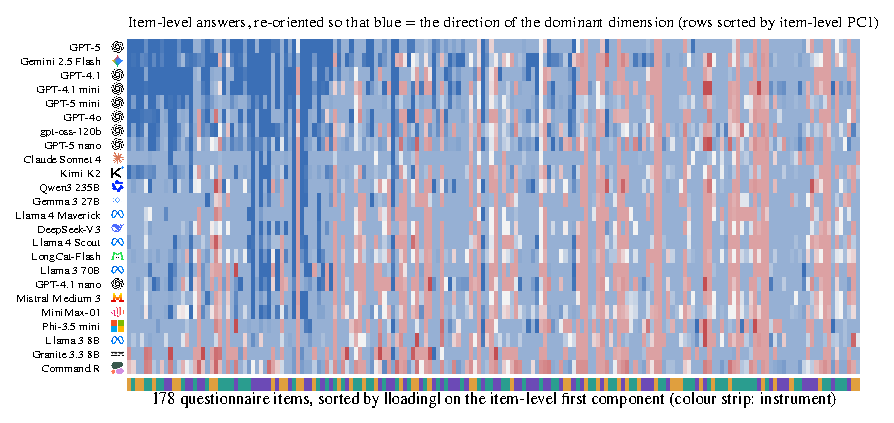
\includegraphics[width=\textwidth]{figures/fig_items.pdf}
\vspace{-6mm}
\caption{\textbf{The gradient is visible in the raw answers.} Mean answers of \nNModels{} models (rows) to all \nNItems{} items (columns). Each item is re-oriented so that blue means agreement in the direction of the dominant item-level component and red the opposite. Columns are sorted by the strength of their loading; the strip below marks the instrument (\instPCT{PCT}, \instSAP{SapplyValues}, \instEV{8Values}). Rows are sorted by item-level PC1. Items from all three instruments are interleaved along the gradient.}
\label{fig:items}
\vspace{-3mm}
\end{figure*}

\begin{table*}[t]
\centering
\small
\begin{tabular}{@{}lp{0.76\textwidth}r@{}}
\toprule
\textbf{Inst.} & \textbf{Item} & \textbf{Lean} \\
\midrule
\tabinput{tables/tab_unanimous.tex}
\bottomrule
\end{tabular}
\caption{The \nNUnanItems{} consensus items, sorted by lean. \swatch{hlAuth}~consensus items whose shared answer pushes the score toward the right/authoritarian/conservative pole.}
\label{tab:unanimous}
\end{table*}


The item-level PCA (Figure~\ref{fig:items}) uses the $\nNModels\times\nNItems$ matrix of mean responses on the $-2$ to $+2$ scale (items with zero variance removed), standardised by column. The permutation null permutes each column independently (500 times).

\paragraph{Interpretation.} The first component explains \nItemPCOne\% of the variance, against \nItemPerm\% expected by chance; the second explains \nItemPCTwo\%. \nItemNRetained{} components exceed the null in total, so the items carry finer structure than the nine named axes. However, the first item-level component correlates $r=\nItemRAxis$ with the axis-level PC1, so the dominant signal is the same at both levels. \nConsUnan{} of the \nNItems{} items receive the same direction of answer from all \nNModels{} models.


\section{t-SNE: A Non-Linear Check}
\label{app:tsne}

The principal component analysis of \S\ref{sec:dimensionality} is linear: it could miss structure that is curved or clustered. As a non-linear check we embed all \nTsneN{} individual runs (the \nNModelsMulti{} models with repeated runs $\times$ 10) with t-SNE, using two feature sets. The first is the nine axis scores (standardised). The second is the raw answers to all \nNItems{} items on the $-2$ to $+2$ scale, which uses no scoring keys at all. Figures~\ref{fig:tsne_axes} and~\ref{fig:tsne_items} show 2-D embeddings (perplexity 30). Each dot is one run, coloured by its model's PC1 score, and each logo sits at its model's centroid. t-SNE preserves local neighbourhoods but not global distances, so we read the maps quantitatively with two statistics, each averaged over five random seeds and two perplexities (10 and 30). \emph{Neighbour purity} is the share of each run's five nearest neighbours in the 2-D map that come from the same model (chance: \nTsnePurChance\%). \emph{Ordering agreement} is the absolute Spearman correlation between a 1-D t-SNE embedding of the model centroids and their PC1 scores.

\begin{figure}[t]
\centering
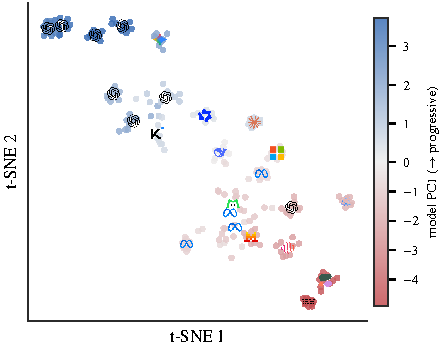
\includegraphics[width=\columnwidth]{figures/fig_tsne_axes.pdf}
\caption{t-SNE of \nTsneN{} runs described by their nine axis scores. Runs are coloured by their model's PC1 score (blue: progressive, egalitarian, libertarian; red: the opposite). The models line up along a single diagonal gradient.}
\label{fig:tsne_axes}
\end{figure}

\begin{figure}[t]
\centering
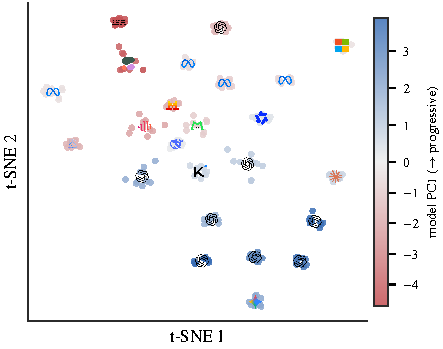
\includegraphics[width=\columnwidth]{figures/fig_tsne_items.pdf}
\caption{t-SNE of the same runs described by their raw answers to all \nNItems{} items, without scoring keys. Each model forms a tight cluster of its own, and the PC1 colour gradient runs across the clusters.}
\label{fig:tsne_items}
\end{figure}

\paragraph{Interpretation.} With axis scores, \nTsnePurAxes\% of each run's neighbours come from the same model, and the 1-D ordering of models agrees with PC1 at $|\rho|=\nTsneRhoAxes$ (range \nTsneRhoAxesLo--\nTsneRhoAxesHi\ across seeds and perplexities). A non-linear method therefore recovers the same single gradient as the linear one, and finds no separate cluster structure that PCA missed. With raw item answers, same-model purity rises to \nTsnePurItems\%: a model's answers act as a stable fingerprint even across runs at temperature 0.6. The ordering still follows PC1 ($|\rho|=\nTsneRhoItems$, range \nTsneRhoItemsLo--\nTsneRhoItemsHi). The lower agreement reflects model-specific detail in the raw answers beyond the shared gradient, consistent with the additional weak components in the item-level PCA (Appendix~\ref{app:items}).

\section{The Multitrait--Multimethod Matrix}
\label{app:mtmm}
\begin{table*}[t]
\centering
\small
\setlength{\tabcolsep}{5pt}
\begin{tabular}{@{}lrcccccrc@{}}
\toprule
\textbf{Model} & $n$ & \textbf{AUC} & \textbf{Within-story conc.} & \textbf{Macro-F1} & $\rho$ & \textbf{Slope} & \textbf{Offset} & \textbf{MAE} \\
\midrule
\tabinput{tables/tab_news_models.tex}
\bottomrule
\end{tabular}
\caption{News slant rating per model, sorted by within-story concordance. \swatch{hlGood}/\swatch{hlWarn}: best/worst value in each column. \swatch{hlLeft}: largest leftward offset. \swatch{hlRight}: the only models with a rightward offset.}
\label{tab:news_models}
\end{table*}


Table~\ref{tab:mtmm_full} shows the full MTMM matrix behind Figure~\ref{fig:mtmm}. Rows and columns are the eight trait-oriented scales: three traits (economic left, libertarian, progressive), each measured by up to three instruments. Each cell gives Spearman's $\rho$ across the \nNModels{} models (bold), its 95\% bootstrap confidence interval, and the FDR-adjusted $p$-value.


\paragraph{Interpretation.} Only \nNConvSig{} of the \nNConv{} same-trait pairs agree significantly: the two progressivism scales, PCT-social with \ev-liberty, and \ev-economic with both other economic scales. \sap's authority scale agrees with neither of its counterparts. Meanwhile \nNViolations{} different-trait pairs reach or exceed a same-trait benchmark. The strongest are \ev-liberty with both progressivism scales ($\rho=\nRhoLibProgSap$ and \nRhoLibProgEight). The others are two within-instrument pairs (PCT economic with PCT social, \ev-economic with \ev-progress) and one involving \sap authority, whose best same-trait correlation is near zero. The block of red cells in the lower right is the conflation of liberty and progressivism described in \S\ref{sec:mtmm}.


\section{Decision Models: Details}
\label{app:decision}

\paragraph{Protocol.} We probed every decision model in the OpenRouter catalogue in November 2026 through its Decisions API. Cloudflare Clairic rejected every question type and is omitted. For each item, the input (\emph{state}) is the statement, and one \emph{choice} question states which instrument the item belongs to and asks for a rating on its agreement scale; the options are the instrument's own labels (four for \pct, five for \sap and \ev, with neutral to be used only when the statement cannot be judged). In the yes/no format each option becomes a separate yes/no question (``Is the rating \emph{strongly agree}?''), and the probabilities are renormalised to sum to one. Responses are deterministic, so each item was asked once per format. The whole study cost US\$0.25.

\begin{table*}[t]
\centering
\small
\setlength{\tabcolsep}{4pt}
\renewcommand{\arraystretch}{1.05}
\begin{tabular}{@{}llrrrrcccc@{}}
\toprule
& & \multicolumn{2}{c}{\textbf{PCT, most likely}} & \multicolumn{2}{c}{\textbf{PCT, expected}} & & & \multicolumn{2}{c}{\textbf{Choice vs.\ yes/no}} \\
\cmidrule(lr){3-4}\cmidrule(lr){5-6}\cmidrule(l){9-10}
\textbf{Model} & \textbf{Developer} & Econ. & Social & Econ. & Social & \textbf{Top $p$} & \textbf{$P$(n)\,\%} & Same top\,\% & $\rho$ \\
\midrule
\tabinput{tables/tab_dec_models.tex}
\bottomrule
\end{tabular}
\caption{All \nDNModels{} decision models, sorted by PCT social score (most libertarian first). \emph{Most likely}: the PCT score of each model's most likely answers. \emph{Expected}: the expected score under its answer distribution. \emph{Top $p$}: mean probability of the most likely option over all \nNItems{} items. \emph{$P$(n)}: mean probability of ``neutral'' on the five-point instruments. \emph{Choice vs.\ yes/no}: share of items with the same most likely answer in the two formats, and Spearman $\rho$ between the expected answers. $^\ddagger$Yes/no format only. \swatch{hlGood}~top $p\geq0.6$. \swatch{hlWarn}~$P$(n)\,$\geq$\,50\% or $\rho<0.6$.}
\label{tab:dec_models}
\end{table*}



\begin{figure*}[t]
\centering
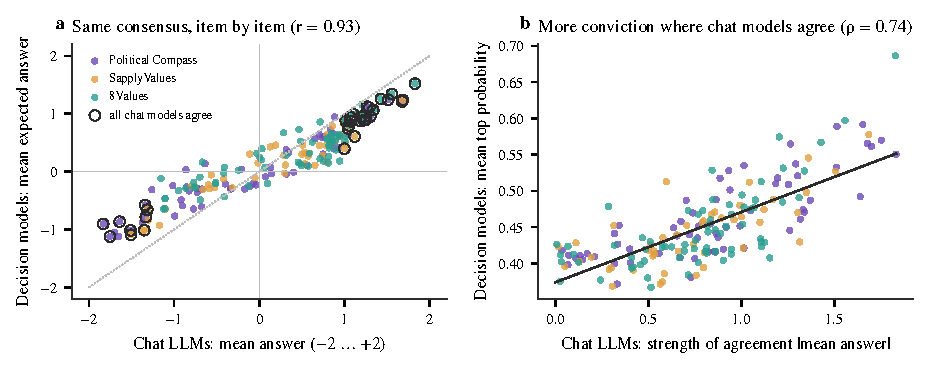
\includegraphics[width=\textwidth]{figures/fig_dec_items.pdf}
\vspace{-6mm}
\caption{\textbf{Decision models share the chat models' consensus.} (a) For each of the \nNItems{} items, the chat LLMs' mean answer against the decision models' mean expected answer ($-2$ to $+2$). Circled: items all chat models answer on the same side. (b) The decision models' mean probability for their most likely option rises with how strongly chat models agree on the item.}
\label{fig:dec_items}
\end{figure*}

\begin{table*}[t]
\centering
\begin{minipage}[t]{0.485\textwidth}
\centering
\footnotesize
\setlength{\tabcolsep}{3pt}
\renewcommand{\arraystretch}{1.02}
\resizebox{\linewidth}{!}{%
\begin{tabular}{@{}lccc@{}}
\toprule
& \textbf{Chat} & \multicolumn{2}{c}{\textbf{\textcolor{cDec}{Decision}}} \\
\cmidrule(l){3-4}
\textbf{Pair} & & expected & answer \\
\midrule
\tabinput{tables/tab_mtmm_rep.tex}
\bottomrule
\end{tabular}}
\caption{The MTMM matrix in both populations: Spearman $\rho$ for all 28 pairs of trait-oriented scales, for chat LLMs ($n=\nNModels$) and decision models ($n=\nDNComplete$; expected and most-likely-answer scores). \swatch{hlRight}~different-trait correlation at least as high as the strongest same-trait one in that column. \swatch{hlWarn}~same-trait correlation below 0.3.}
\label{tab:mtmm_rep}
\end{minipage}\hfill
\begin{minipage}[t]{0.485\textwidth}
\centering
\footnotesize
\setlength{\tabcolsep}{3pt}
\resizebox{\linewidth}{!}{%
\begin{tabular}{@{}lcc@{}}
\toprule
\textbf{Quantity} & \textbf{\nNModels} & \textbf{All \nNModelsAll} \\
\midrule
\tabinput{tables/tab_sensitivity.tex}
\bottomrule
\end{tabular}}
\caption{Main results for the \nNModels{} same-protocol models and for all \nNModelsAll{} chat models (news correlations: \nNModelsLink{} and \nNModelsNews{} models). \swatch{hlWarn}~values that change qualitatively.}
\label{tab:sensitivity}

\vspace{4mm}
\footnotesize
\setlength{\tabcolsep}{2.6pt}
\resizebox{\linewidth}{!}{%
\begin{tabular}{@{}lrrrrrrr@{}}
\toprule
\textbf{Model} & $n$ & AUC & Conc. & Slope & Offset & Top $p$ & PC1 \\
\midrule
\tabinput{tables/tab_dec_news.tex}
\bottomrule
\end{tabular}}
\caption{News slant rating by the \nDNNews{} decision models, sorted by within-story concordance. Metrics as in Table~\ref{tab:news_models}; \emph{Top $p$}: mean probability of the most likely slant level; \emph{PC1}: questionnaire ideology score (expected answers). \swatch{hlGood}~concordance $\geq0.70$ or AUC $\geq0.78$. \swatch{hlRight}~positive offset. $^{\S}$Articles blocked by the provider's content filter excluded.}
\label{tab:dec_news}
\end{minipage}
\end{table*}

\paragraph{Interpretation.} Table~\ref{tab:dec_models} shows the same spread as among chat models. The Liquid models, Gemini Decision-1 and Perplexity's Decider Flash sit far in the libertarian-left corner, and Joey-1 is the one model outside it, just above the economic axis. Scoring by expected answers moves every model toward the centre, most strongly the models with diffuse distributions: \nDShrinkMinModel{} keeps only \nDShrinkMin\% of its distance from the origin. The exception is Span-01, the only model asked in the yes/no format. Conviction is generally low; only the two Upstage models, Span-01 and GPT-6 Luna Decisions reach a mean top probability of 0.6. The Upstage models reach it mainly by putting most of their probability on ``neutral'', so their high conviction is a refusal to take sides, and they are also the least stable across formats ($\rho\leq0.55$). Classify-1 is the third unstable model.

Table~\ref{tab:mtmm_rep} shows why the replication is informative. In both populations PCT-social converges with \ev-liberty and the progressivism scales converge, \sap authority converges with neither other authority scale, and \ev-liberty correlates with \ev-progress about as strongly as any same-trait pair. Decision models add a strong within-instrument correlation between PCT economic and social. The main difference is \sap-progressive: among chat models it tracks \ev-liberty ($\rho=\nCLibProgSap$), among decision models much less so. Expected scores, which use the full distributions, give higher same-trait correlations than most-likely answers, because they are less affected by ties between neighbouring options. Figure~\ref{fig:dec_items} shows the item-level agreement behind Table~\ref{tab:dec}: the two populations order the \nNItems{} items almost identically, and decision models are most confident on the items that chat models answer unanimously.



\paragraph{News rating.} Table~\ref{tab:dec_news} lists the news metrics of the \nDNNews{} decision models that rated articles. The four best discriminators (D1 Ultra, Gemini Decision-1, D1.1 and D1.2) also have the four highest questionnaire PC1 scores, and two of the three weakest (Joey-1 and TEV1) have the lowest, which is the pattern behind the correlations in Table~\ref{tab:link}. Classify-1, the weakest, sits mid-range. Gemini Decision-1 is the only model that refused articles; the \nGemRefused{} it blocked include \nGemRefFarRight{} of 28 Far Right and \nGemRefRight{} of 131 Right articles, against \nGemRefMid{} of the 845 Center and Lean articles. Topics included the war in Gaza, transgender care for minors and Texas redistricting.

\section{Sensitivity: All \nNModelsAll{} Chat Models}
\label{app:sensitivity}

Table~\ref{tab:sensitivity} repeats the key questionnaire analyses with Grok~4 and Gemini~2.5 Pro included, even though their questionnaires were collected under a different prompt.









\paragraph{Interpretation.} The conclusions hold, with two qualifications. First, a second component now passes the random-data threshold. It is driven almost entirely by Grok~4, the only economically right-of-centre model in the cohort, and so reflects one model, not a second ideological dimension shared across models. Second, the average same-trait correlation is clearly higher than the average different-trait one across instruments (\nSMeanMono{} vs.\ \nSMeanHH), a wider gap than in the main cohort. Even so, the liberty--progressivism correlation ($\rho=\nSRhoLibProgSap$) still exceeds every same-trait correlation in the matrix, so discriminant validity still fails. The decoupling between questionnaire position and news-rating direction is unchanged.


\section{Key-Free Similarity of Answer Vectors}
\label{app:similarity}

All analyses so far rely on the instruments' scoring keys. Here we use none. Each run's answers to an instrument form a vector (strongly agree $=+2$, agree $=+1$, neutral $=0$, disagree $=-1$, strongly disagree $=-2$), and a model's vector is the mean over its runs. We compare vectors with cosine similarity, either on the raw answers or after subtracting each item's cohort mean (\emph{item-centred}), which removes the answers all models share and keeps only how a model departs from them. Table~\ref{tab:similarity} reports three analyses. \emph{Cosine similarity} compares models and runs within each instrument. \emph{RSA} (representational similarity analysis) asks whether two instruments agree on which models resemble each other: we correlate the $\nNModels\times\nNModels$ item-centred similarity matrices of two instruments (Spearman), with $p$-values from 5{,}000 permutations of model labels. \emph{Same-developer excess} is the mean similarity of model pairs from the same developer minus that of pairs from different developers (all \nNItems{} items, item-centred), tested by permuting developer labels. We repeat it leaving out each developer with several models, and after regressing pairwise similarity on the models' distance on PC1.

\begin{table}[t]
\centering
\footnotesize
\setlength{\tabcolsep}{3pt}
\resizebox{\columnwidth}{!}{%
\begin{tabular}{@{}lccc@{}}
\toprule
& \textbf{\pct} & \textbf{\sap} & \textbf{\ev} \\
\midrule
\tabinput{tables/tab_similarity.tex}
\bottomrule
\end{tabular}}
\caption{Key-free similarity analysis (\nNModels{} models). \swatch{hlWarn}~raw similarity dominated by shared answers, and lineage tests that do not hold. \swatch{hlGood}~key-free reliability and the strongest agreement between instruments.}
\label{tab:similarity}
\end{table}

\begin{figure}[t]
\centering
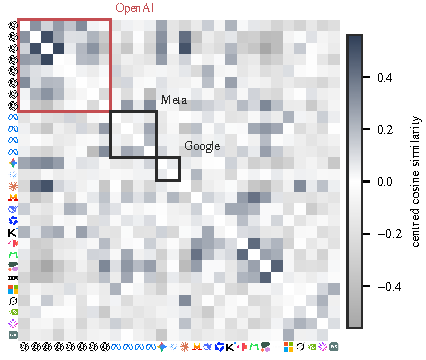
\includegraphics[width=\columnwidth]{figures/fig_similarity.pdf}
\caption{Item-centred cosine similarity between the \nNModels{} models over all \nNItems{} items, sorted by developer (boxes) and, within a developer, by PC1. Dark cells: two models depart from the shared answers in the same way. Only the OpenAI block stands out.}
\label{fig:similarity}
\end{figure}

\paragraph{Interpretation.} Three findings, one of them negative.
\begin{itemize}[leftmargin=*,itemsep=1pt,topsep=2pt]
\item \textbf{Raw similarity is consensus.} Any two models' raw answer vectors are similar (mean cosine \nSimRaw), because they share most of their answers. Once the shared part is removed, similarity between different models falls to about zero, while runs of the same model stay at \nSimRunsWithinLo--\nSimRunsWithinHi. This is a key-free confirmation of the reliability in Table~\ref{tab:reliability}.
\item \textbf{The PCT orders models differently.} \sap and \ev largely agree on which models resemble each other ($\rho=\nRsaSapEv$), whereas the PCT agrees with them only weakly ($\rho=\nRsaPctSap$ and \nRsaPctEv). Because this uses no scoring keys, it independently supports the MTMM result (\S\ref{sec:mtmm}): the PCT captures a different mixture of attitudes than the other two instruments.
\item \textbf{There is no general developer fingerprint.} Same-developer pairs are more similar overall (excess \nLinAll, $p=\nLinAllP$). But \nNOAIPairs{} of the \nNSameDev{} same-developer pairs are OpenAI models, and without them the excess vanishes (\nLinNoOAI, $p=\nLinNoOAIP$). It also shrinks once ideological distance is controlled (\nLinCtrl, $p=\nLinCtrlP$). Figure~\ref{fig:similarity} shows the same: only the OpenAI block is dark. What looks like a lineage effect is an OpenAI house style, partly shared ideology.
\end{itemize}
A hubness measure from cross-lingual embedding alignment (CSLS; mean similarity to a model's five nearest neighbours) was unstable across instruments ($\rho=\nHubLo$--\nHubHi) and tracked distance from the centre of PC1 ($\rho=\nHubAbsPC$), so with \nNModels{} models it reflects membership of a tight cluster, not typicality. We do not interpret it further.

Table~\ref{tab:simpairs} lists every model pair. Only \nTopTenSameDev{} of the ten most similar pairs share a developer. GPT-5 is almost as close to Claude Sonnet~4 ($+0.50$) as to GPT-4.1 ($+0.53$), and Command~R and Granite~3.3, two of the lowest models on PC1, form the closest pair outside the OpenAI--Anthropic group ($+0.45$). The most dissimilar pair is GPT-5 and Command~R ($-0.56$), from opposite ends of PC1. Similarity of answers therefore follows position on the shared ideological gradient more than it follows lineage.

\section{Reference Respondents and Consensus Items}
\label{app:location}

Table~\ref{tab:reference} applies the re-implemented scoring functions (\S\ref{sec:setup}) to hypothetical respondents who give the same answer to every item, and to 10{,}000 simulated respondents who answer uniformly at random. Columns are the same axes as in Table~\ref{tab:models}.


\paragraph{Interpretation.} A random respondent lands at the centre of every axis, so no instrument has a built-in libertarian-left tilt. A respondent who agrees with everything is pushed toward \emph{authority} on PCT social and \ev liberty. These two axes are keyed so that only \nKeyBalPctSoc\% and \nKeyBalEvGovt\% of their item weight, respectively, rewards agreement with the libertarian pole. Since the models agree often, their libertarian placement is reached \emph{against} the pull of response style, not because of it.

\medskip
Table~\ref{tab:unanimous} lists the \nNUnanItems{} items on which all \nNModels{} models answer on the same side. \emph{Lean} is the item's push on its most heavily weighted axis, from $-1$ (all the way to the right/authoritarian/conservative pole) to $+1$ (left/libertarian/progressive), relative to a random respondent (\S\ref{sec:location}).


\paragraph{Interpretation.} The strongest consensus items concern equal treatment, racial superiority, sexuality, religious freedom and scientific consensus (astrology, climate change). The models' shared answer coincides with the left/libertarian/progressive pole on all of them. But the consensus is not one-sided: \nUnanItemsNeg{} items (highlighted) are endorsed by every model and pull the scores toward the other pole. They concern national sovereignty, morally sound authority figures, institutional structure and surveillance of extremists.

\section{Per-Model News Rating Results}
\label{app:news}

Table~\ref{tab:news_models} gives each model's news-rating metrics (\S\ref{sec:news}). $n$ is the number of valid ratings out of \nNArticles. \emph{AUC} measures how well the rating separates left-labelled from right-labelled articles (Center excluded; 0.5 = chance). \emph{Within-story conc.}\ is the share of same-story article pairs with different labels that the model orders like their labels (0.5 = chance). \emph{Macro-F1} is computed over left/centre/right, with ratings beyond $\pm0.5$ counted as left or right (majority baseline \nFOneMaj). $\rho$ is the Spearman correlation between rating and label. \emph{Slope} and \emph{offset} come from a linear fit of rating on label: a perfectly calibrated rater would have slope 1 and offset 0. \emph{MAE} is the mean absolute error, which depends heavily on the compression of the scale.


\paragraph{Interpretation.} \nBestConcModel{} ranks same-story outlets best and \nWorstConcModel{} worst, barely above chance. \nSlopeBelowHalf{} of \nNModelsNews{} models have a slope below 0.5, so compression is universal, not a property of a few weak models. Offsets are small and leftward for all but \nNPosOffset{} models. Phi-3.5~mini is a clear outlier: its large leftward offset comes with weak discrimination, which suggests difficulty with the task, not a distinct political stance.

\section{The Questionnaire Items}
\label{app:allitems}

Tables~\ref{tab:items_pct}--\ref{tab:items_8val} list every statement of the three instruments in their original order, with the instrument's own thematic grouping shown by row colour (a shared colour marks the same theme across instruments). \emph{Agree $\rightarrow$} gives the pole toward which agreeing moves the score, read from the instrument's scoring key: \emph{Left/Right}, \emph{Lib./Auth.} (libertarian/authoritarian), \emph{Prog./Cons.} or \emph{Prog./Trad.} (progressive/conservative or traditional), \emph{Equal./Mkt.} (equality/markets) and \emph{Glob./Nat.} (globalist/nationalist). Several \ev items move more than one axis. \emph{Mean} is the \nNModels{} models' average answer on a $-2$ (strongly disagree) to $+2$ (strongly agree) scale; the PCT has no neutral option. \emph{Cons.}\ is the share of models whose average answer falls on the majority side, and $\bigstar$ marks items on which all \nNModels{} models agree in direction.

\paragraph{Interpretation.} Models agree with \nItemsAgreeShare\% of the \nNItems{} statements on average. Their answers are strong in both directions: \nItemsStrongAgree{} statements receive a mean of at least $+1$ and \nItemsStrongDisagree{} a mean of at most $-1$. The tables make the patterns of \S\ref{sec:location} visible item by item. The models agree with qualified statements whichever pole they point to; for example, they support both ``the freer the markets, the freer the people'' and government intervention to protect consumers (\ev items 3 and 2). They reject absolute or discriminatory claims. The \emph{Agree $\rightarrow$} column also shows the keying imbalance: most PCT social items are worded so that agreeing is authoritarian, so the models' libertarian placement comes mostly from \emph{disagreeing}.







\begin{table*}[p]
\centering
\small
\setlength{\tabcolsep}{4pt}
\renewcommand{\arraystretch}{1.08}
\begin{tabular}{@{}r p{0.68\textwidth} p{0.11\textwidth} r r@{}}
\toprule
\textbf{\#} & \textbf{Political Compass statement} & \textbf{Agree$\rightarrow$} & \textbf{Mean} & \textbf{Cons.} \\
\midrule
\tabinput{tables/tab_items_pct_1.tex}
\bottomrule
\end{tabular}
\caption{The 62 Political Compass statements. Rows are coloured by the test's own six thematic blocks: \swatch{catD}~country and world, \swatch{catA}~economy, \swatch{catB}~personal social values, \swatch{catC}~wider society, \swatch{catE}~religion and \swatch{catF}~sex. Item 21 has no effect on either score in the scoring code (\emph{unscored}).\label{tab:items_pct}}
\end{table*}

\begin{table*}[p]
\centering
\small
\setlength{\tabcolsep}{4pt}
\renewcommand{\arraystretch}{1.08}
\begin{tabular}{@{}r p{0.68\textwidth} p{0.11\textwidth} r r@{}}
\toprule
\textbf{\#} & \textbf{Political Compass statement} & \textbf{Agree$\rightarrow$} & \textbf{Mean} & \textbf{Cons.} \\
\midrule
\tabinput{tables/tab_items_pct_2.tex}
\bottomrule
\end{tabular}
\captionsetup{list=false}\caption*{Political Compass statements (continued from Table~\ref{tab:items_pct}).}
\end{table*}

\begin{table*}[p]
\centering
\small
\setlength{\tabcolsep}{4pt}
\renewcommand{\arraystretch}{1.08}
\begin{tabular}{@{}r p{0.68\textwidth} p{0.11\textwidth} r r@{}}
\toprule
\textbf{\#} & \textbf{SapplyValues statement} & \textbf{Agree$\rightarrow$} & \textbf{Mean} & \textbf{Cons.} \\
\midrule
\tabinput{tables/tab_items_sap_1.tex}
\bottomrule
\end{tabular}
\caption{The 46 SapplyValues statements, coloured by axis: \swatch{catA}~economic (left/right), \swatch{catB}~authority (libertarian/authoritarian) and \swatch{catC}~progressivism (progressive/conservative).\label{tab:items_sap}}
\end{table*}

\begin{table*}[p]
\centering
\small
\setlength{\tabcolsep}{4pt}
\renewcommand{\arraystretch}{1.08}
\begin{tabular}{@{}r p{0.68\textwidth} p{0.11\textwidth} r r@{}}
\toprule
\textbf{\#} & \textbf{8Values statement} & \textbf{Agree$\rightarrow$} & \textbf{Mean} & \textbf{Cons.} \\
\midrule
\tabinput{tables/tab_items_8val_1.tex}
\bottomrule
\end{tabular}
\caption{The 70 8Values statements, coloured by the axis each item weights most heavily: \swatch{catA}~economic (equality/markets), \swatch{catD}~diplomatic (globalism/nationalism), \swatch{catB}~civil (liberty/authority) and \swatch{catC}~societal (progress/tradition).\label{tab:items_8val}}
\end{table*}

\begin{table*}[p]
\centering
\small
\setlength{\tabcolsep}{4pt}
\renewcommand{\arraystretch}{1.08}
\begin{tabular}{@{}r p{0.68\textwidth} p{0.11\textwidth} r r@{}}
\toprule
\textbf{\#} & \textbf{8Values statement} & \textbf{Agree$\rightarrow$} & \textbf{Mean} & \textbf{Cons.} \\
\midrule
\tabinput{tables/tab_items_8val_2.tex}
\bottomrule
\end{tabular}
\captionsetup{list=false}\caption*{8Values statements (continued from Table~\ref{tab:items_8val}).}
\end{table*}


\begin{table*}[p]
\centering
\footnotesize
\setlength{\tabcolsep}{3.3pt}
\renewcommand{\arraystretch}{1.0}
\begin{tabular}{@{}rllrrrrr@{}}
\toprule
& & & & \multicolumn{4}{c}{\textbf{Item-centred cosine similarity}} \\
\cmidrule(l){5-8}
\textbf{\#} & \textbf{Model A} & \textbf{Model B} & \textbf{Same developer} & \textbf{All items} & \pct & \sap & \ev \\
\midrule
\tabinput{tables/tab_simpairs_1.tex}
\bottomrule
\end{tabular}
\caption{All \nNPairsSim{} model pairs, sorted by item-centred cosine similarity over all \nNItems{} items (the values in Figure~\ref{fig:similarity}), with the same similarity computed within each instrument. \swatch{catD}~pairs from the same developer. Bold: $|$similarity$|\geq0.40$.\label{tab:simpairs}}
\end{table*}

\begin{table*}[p]
\centering
\footnotesize
\setlength{\tabcolsep}{3.3pt}
\renewcommand{\arraystretch}{1.0}
\begin{tabular}{@{}rllrrrrr@{}}
\toprule
& & & & \multicolumn{4}{c}{\textbf{Item-centred cosine similarity}} \\
\cmidrule(l){5-8}
\textbf{\#} & \textbf{Model A} & \textbf{Model B} & \textbf{Same developer} & \textbf{All items} & \pct & \sap & \ev \\
\midrule
\tabinput{tables/tab_simpairs_2.tex}
\bottomrule
\end{tabular}
\caption*{All model pairs by similarity (continued from Table~\ref{tab:simpairs}).}
\end{table*}

\begin{table*}[p]
\centering
\footnotesize
\setlength{\tabcolsep}{3.3pt}
\renewcommand{\arraystretch}{1.0}
\begin{tabular}{@{}rllrrrrr@{}}
\toprule
& & & & \multicolumn{4}{c}{\textbf{Item-centred cosine similarity}} \\
\cmidrule(l){5-8}
\textbf{\#} & \textbf{Model A} & \textbf{Model B} & \textbf{Same developer} & \textbf{All items} & \pct & \sap & \ev \\
\midrule
\tabinput{tables/tab_simpairs_3.tex}
\bottomrule
\end{tabular}
\caption*{All model pairs by similarity (continued from Table~\ref{tab:simpairs}).}
\end{table*}

\begin{table*}[p]
\centering
\footnotesize
\setlength{\tabcolsep}{3.3pt}
\renewcommand{\arraystretch}{1.0}
\begin{tabular}{@{}rllrrrrr@{}}
\toprule
& & & & \multicolumn{4}{c}{\textbf{Item-centred cosine similarity}} \\
\cmidrule(l){5-8}
\textbf{\#} & \textbf{Model A} & \textbf{Model B} & \textbf{Same developer} & \textbf{All items} & \pct & \sap & \ev \\
\midrule
\tabinput{tables/tab_simpairs_4.tex}
\bottomrule
\end{tabular}
\caption*{All model pairs by similarity (continued from Table~\ref{tab:simpairs}).}
\end{table*}

\begin{table*}[p]
\centering
\footnotesize
\setlength{\tabcolsep}{3.3pt}
\renewcommand{\arraystretch}{1.0}
\begin{tabular}{@{}rllrrrrr@{}}
\toprule
& & & & \multicolumn{4}{c}{\textbf{Item-centred cosine similarity}} \\
\cmidrule(l){5-8}
\textbf{\#} & \textbf{Model A} & \textbf{Model B} & \textbf{Same developer} & \textbf{All items} & \pct & \sap & \ev \\
\midrule
\tabinput{tables/tab_simpairs_5.tex}
\bottomrule
\end{tabular}
\caption*{All model pairs by similarity (continued from Table~\ref{tab:simpairs}).}
\end{table*}

\begin{table*}[p]
\centering
\footnotesize
\setlength{\tabcolsep}{3.3pt}
\renewcommand{\arraystretch}{1.0}
\begin{tabular}{@{}rllrrrrr@{}}
\toprule
& & & & \multicolumn{4}{c}{\textbf{Item-centred cosine similarity}} \\
\cmidrule(l){5-8}
\textbf{\#} & \textbf{Model A} & \textbf{Model B} & \textbf{Same developer} & \textbf{All items} & \pct & \sap & \ev \\
\midrule
\tabinput{tables/tab_simpairs_6.tex}
\bottomrule
\end{tabular}
\caption*{All model pairs by similarity (continued from Table~\ref{tab:simpairs}).}
\end{table*}

\begin{table*}[p]
\centering
\footnotesize
\setlength{\tabcolsep}{3.3pt}
\renewcommand{\arraystretch}{1.0}
\begin{tabular}{@{}rllrrrrr@{}}
\toprule
& & & & \multicolumn{4}{c}{\textbf{Item-centred cosine similarity}} \\
\cmidrule(l){5-8}
\textbf{\#} & \textbf{Model A} & \textbf{Model B} & \textbf{Same developer} & \textbf{All items} & \pct & \sap & \ev \\
\midrule
\tabinput{tables/tab_simpairs_7.tex}
\bottomrule
\end{tabular}
\caption*{All model pairs by similarity (continued from Table~\ref{tab:simpairs}).}
\end{table*}

\end{document}
